% !TeX spellcheck = es_ES
% !TEX encoding = UTF-8 Unicode
\documentclass[t, compress, spanish, aspectratio=169]{beamer}
%\documentclass[handout]{beamer}    % for the handout

\usetheme[progressbar=frametitle]{metropolis}

%\usetheme[secheader]{Madrid}
%\usetheme{Frankfurt}
%\usetheme{Warsaw}
%\usetheme{Berlin}
%\usetheme{CambridgeUS}

%\usecolortheme{beaver}     % Fondo Blanco y letras Negras - Titulos en Rojo con fondo gris
%\usecolortheme{dove}       % Para el Handout
%\usecolortheme{seahorse}   % Fondo Blanco y letras Negras - Titulos en Celeste
%\usecolortheme{dolphin}    % Fondo Blanco y letras Negras - Titulos en Celeste
%\usecolortheme{seagull}    % Fondo Blanco y letras Negras - Titulos en Gris
%\usecolortheme{crane}      % Fondo Blanco y letras Negras - Titulos en Amarillo
%\usecolortheme{wolverine}  % Fondo Blanco y Letras negras - Titulos en negro con fondo amarillo
%\usecolortheme{lily}       % Fondo Blanco y letras Negras - Titulos en Azul
%\usecolortheme{fly}        % Fondo Gris y letras Negras - Titulos en Rojo
%\usecolortheme{beetle}     % Fondo Gris y letras Negras - Titulos en blanco
%\usecolortheme{albatross}  % Fondo Azul y letras blancas
%\usecolortheme{orchid}     % Default
%\usecolortheme{rose}       % Default
%\usecolortheme{whale}      % Default

\setbeamertemplate{navigation symbols}{} % Gets rid of navigation symbols
%\setbeamercovered{transparent}

\usepackage{dsfont} % Double stroke fonts for math symbols
% \usepackage[T1]{fontenc}  % Helps with hyphenation for languages with accented characters. Note: Does not work with XeLaTex
% \usepackage[latin1]{inputenc} % Allows to type in latin (accents). Note: Does not work with XeLaTex
% \usefonttheme[onlymath]{serif}  % Changes fonts for math to serif
\usepackage[english]{babel} % Manages differences between languages: hyphenation etc

\usepackage{appendixnumberbeamer} % Does not include backup slides in the number of pages

\usepackage{centernot} % To draw not in math symbols (does not imply)

\usepackage{ragged2e}  % Text alignment
\justifying

\usepackage{graphicx} % Format for graphics: additional options for includefigure
\usepackage{pgf} % Tool for graphics

\usepackage{booktabs} % Format for tables: top, bottom and mid lines
\usepackage[scale=2]{ccicons}
\usepackage{threeparttable} % Format for tables
\usepackage{lscape} % Landscape for tables

% Customized commands
  \newcommand{\vs}{\vskip0pt plus.5fill}
  \newcommand{\SR}{\mathbb{R}}
  \DeclareMathOperator{\plim}{plim}
  \DeclareMathOperator{\Var}{Var}
  \DeclareMathOperator{\Avar}{AVar}
  \DeclareMathOperator{\Cov}{Cov}
  \DeclareMathOperator{\N}{Normal}
  \DeclareMathOperator{\E}{\mathbb{E}}
  \DeclareMathOperator{\LP}{\mathbb{L}}
  \newcommand{\pto}{\stackrel{p}{\longrightarrow}}
  \newcommand{\dto}{\stackrel{d}{\longrightarrow}}
  \newcommand{\adistr}{\stackrel{a}{\sim}}
  \newcommand{\epsi}{\varepsilon}
  \newcommand{\tmle}{\hat \theta_{ML}}
  \newcommand{\tgmm}{\hat \theta_{GMM}}
  \newcommand\independent{\protect\mathpalette{\protect\independenT}{\perp}}
  \def\independenT#1#2{\mathrel{\rlap{$#1#2$}\mkern2mu{#1#2}}}

\title [Variables instrumentales y 2SLS] {Econometr\'ia I \\ 
	Variables instrumentales y M\'inimos cuadrados en dos etapas (2SLS)}
\author[de Elejalde]{Ramiro de Elejalde}
\institute [UAH] {Facultad de Econom\'ia y Finanzas \\ Universidad Alberto Hurtado}
\date[\today] {}
\subject{Econometr\'ia}
\begin{document}
	
	%------------------------------------------------------------
	\begin{frame}
		\titlepage
	\end{frame}
	% --------------------------------------------------- Slide --
	\begin{frame}
		\frametitle{Outline}
		\scriptsize
		\tableofcontents
		\alert{Referencias}: Cap. 4 de Angrist and Pischke, cap. 5 de Wooldridge, y cap. 12 de Stock and Watson.
	\end{frame}
	% --------------------------------------------------- Slide --
	\section{Modelo simple}
	\begin{frame}
		\frametitle{Modelo simple}
			\begin{align*}
			y_i=\beta_0 + \beta_1 x_{i}+u_i,
			\end{align*}
			donde $y_i$ es la variable dependiente, $x_i$ es una variable \alert{end\'ogena} y $z_i$ es un \alert{instrumento}.
			
			Supuestos: $\Cov(x_i,u_i) \neq 0$ ($x_i$ es end\'ogena)
			\begin{enumerate}
				\bigskip
				\item [IV1] Muestra aleatoria de tama\~no $N$ $\implies \{y_i,x_i,z_i\}_{i=1}^N$ i.i.d.,
				\bigskip
				\item [IV2]  \alert{Exogeneidad del instrumento} (Restricci\'on de exclusi\'on): $\Cov(z_i,u_i)=0$,\\
				Dos condiciones: (1) $z_i$ es \emph{como si fuese} asignada en forma aleatoria,  (2) $z_i$ no tiene un efecto directo sobre $y_i$.
				\bigskip
				\item [IV3]  \alert{Relevancia del instrumento}: $\Cov(z_i,x_i)\neq 0$
				\bigskip
			\end{enumerate}
	\end{frame}
	% --------------------------------------------------- Slide --
	
%	\begin{frame}
%		\frametitle{Modelo simple}
%	\end{frame}
%			
%	\begin{frame}
%		\frametitle{Modelo simple}
%	\end{frame}

	\begin{frame}
		\frametitle{Efecto de la fertilidad en la oferta laboral (Angrist y Evans, AER 1998)}
		\begin{itemize}
			\item  ?`Cu\'al es el efecto de tener hijos en la oferta laboral de las mujeres?
			\item  Datos: Census Public Use Micro Sample (PUMS) para 1980 y 1990.
			\item  Muestra: Una muestra con mujeres casadas con al menos 2 hijos.
			\item  \alert{Variable dependiente}: estar empleada ($workedm$), semanas trabajadas ($weeksm1$) y horas trabajadas por semana ($hourswm$).
			\item  \alert{Variable explicativa}: Tener 3 hijos o m\'as ($morekids$).
			\item  \alert{Instrumentos}: Hijos del mismo sexo ($samesex$).
		\end{itemize}
	\end{frame}
	% --------------------------------------------------- Slide --
	\begin{frame}
		\frametitle{Efecto de la fertilidad en la oferta laboral (Angrist y Evans, AER 1998)}
		\begin{itemize}
			\item  ?`El hecho que los dos primeros dos hijos sean del mismo sexo ($samesex$) es un buen instrumento para tener tres hijos o m\'as ($morekids$)?
			\item  <2-> \alert{Exogeneidad}
			\begin{itemize}
				\item <2->?`Es el sexo de los hijos asignado aleatoriamente?
				\item <2-> ?`El sexo de los hijos puede estar correlado con la decisi\'on de trabajar de la madre por razones distintas de su efecto sobre el n\'umero de ni\~nos?
			\end{itemize}
			\item  <2-> \alert{Relevancia}: ?`Tener dos hijos del mismo sexo afecta la decisi\'on de tener un hijo adicional? 
			\begin{itemize}
				\item <2-> Se puede inferir de los datos.
			\end{itemize}    
		\end{itemize}
	\end{frame}
	% --------------------------------------------------- Slide --
	\subsection{Identificaci\'on}
	\begin{frame}
		\frametitle{Identificaci\'on}
		\begin{itemize}
			\item  ?`Qu\'e momentos poblacionales permiten identificar los par\'ametros de inter\'es?
			\item [] <2->
			\begin{align*}
				&\Cov(z_i,u_i)=0 \quad \text{usando IV2},\\
				&\iff \Cov(z_i(y_i-\beta_0-\beta_1x_i)) =0,\\
				&\iff \Cov(z_i,y_i)-\beta_1\Cov(z_i,x_i) =0,\\
				&\iff \alert{\beta_1 =\frac{\Cov(z_i,y_i)}{\Cov(z_i,x_i)}}\quad \text{usando IV3}.
			\end{align*}
			\item  <3-> IV2 y IV3 son los supuestos que identifican a $\beta_1$.
		\end{itemize}
	\end{frame}
	% --------------------------------------------------- Slide --
%	\begin{frame}
%		\frametitle{M\'inimos Cuadrados Indirectos}
%	\end{frame}
%	
%	\begin{frame}
%		\frametitle{M\'inimos Cuadrados Indirectos}
%	\end{frame}
			
	% --------------------------------------------------- Slide --
	\begin{frame}
		\frametitle{M\'inimos Cuadrados Indirectos}
		\begin{itemize}
			\item \alert{Primera etapa}
			\begin{align*}
				x_i=\pi_{10}+\pi_{11}z_i+\epsilon_{1i}.
			\end{align*}
			\item \alert{Forma reducida}
			\begin{align*}
				y_i=\pi_{20}+\pi_{21}z_i+\epsilon_{2i}.
			\end{align*}
			\item  [] Entonces,
			\begin{align*}
				\beta_1&=\frac{\Cov(z_i,y_i)}{\Cov(z_i,x_i)},\\
				&=\frac{\Cov(z_i,y_i)/\Var(z_i)}{\Cov(z_i,x_i)/\Var(z_i)},\\
				\implies \alert{\beta_1}&\alert{=\frac{\pi_{21}}{\pi_{11}} }.
			\end{align*}
			\item Intuici\'on: Correlaci\'on entre $z_i$ e $y_i$ solamente se puede deber al efecto a trav\'es de $x_i$.
		\end{itemize}
	\end{frame}
	% --------------------------------------------------- Slide --
%	\begin{frame}
%		\frametitle{M\'inimos Cuadrados en 2 Etapas (2SLS)}
%	\end{frame}
%	
%	\begin{frame}
%		\frametitle{M\'inimos Cuadrados en 2 Etapas (2SLS)}
%	\end{frame}	

	% --------------------------------------------------- Slide --
	\begin{frame}
		\frametitle{M\'inimos Cuadrados en 2 Etapas (2SLS)}
		\begin{itemize}
			\item \alert{Primera etapa}
			\begin{align*}
				x_i=\pi_{10}+\pi_{11}z_i+\epsilon_{1i}=x_i^*+\epsilon_{1i}.
			\end{align*}
			\item  Luego reemplazar $x_i$ por la predicci\'on $x_i^*$ (que no est\'a correlada con el error).
			\begin{align*}
				y_i&=\beta_{0}+\beta_1 x_i+u_{i},\\
				&=\beta_{0}+\beta_1x_i-\beta_1 x_i^*+\beta_1 x_i^*+u_{i},\\
				&=\beta_{0}+\beta_1 x_i^*+\beta_1(x_i-x_i^*)+u_{i}.
			\end{align*}
			\item  [] Entonces,
			\begin{align*}
				\alert{ \beta_{1}=\frac{\Cov(x_i^*,y_i)}{\Var(x_i^*)} }.
			\end{align*}
			\item Intuici\'on: Solamente utilizamos la variaci\'on ex\'ogena de $x_i$.
		\end{itemize}
	\end{frame}
%	% --------------------------------------------------- Slide --
%	\begin{frame}
%		\frametitle{Caso especial: Estimador de Wald}
%	\end{frame}
%
%	\begin{frame}
%		\frametitle{Caso especial: Estimador de Wald}
%		\begin{itemize}
%			\item  En el modelo
%			\begin{align*}
%				y_i=\beta_0 + \beta_1 x_{i}+u_i,
%			\end{align*}
%			con $z_i$ un instrumento v\'alido.
%			\item  Supongamos que el instrumento es una variable binaria tal que
%			\begin{align*}
%				z_i=\left\{
%				\begin{array}{c l}
%					1 & \text{con probabilidad } p\\
%					0 & \text{con probabilidad } 1-p                 
%				\end{array}
%				\right.
%			\end{align*}
%			\item  [] Entonces el estimador IV es igual al llamado estimado de Wald:
%			\begin{align*}
%				\beta_{1, Wald}=\frac{\E(y|z=1)-\E(y|z=0)}{\E(x|z=1)-\E(x|z=0)}
%			\end{align*}
%		\end{itemize}
%	\end{frame}
%	% --------------------------------------------------- Slide --
%	\begin{frame}
%		\frametitle{Estimador de Wald}
%	\end{frame}
%	% --------------------------------------------------- Slide --
%	\begin{frame}
%		\frametitle{Estimador de Wald}
%	\end{frame}
%	% --------------------------------------------------- Slide --
%	\begin{frame}
%		\frametitle{Estimador de Wald}
%		\begin{itemize}
%			\item  \alert{El estimador de Wald es un estimador IV}: $\beta_{1,Wald}=\beta_{1,IV}$
%			\item  [] Demostraci\'on: Utilice la LEI para escribir
%			\small
%			\begin{align*}
%				\E(y) &= \E[\E(y|z)]= (1-p) \E(y|z=0)+ p \E(y|z=1), \\
%				\E(zy) &= \E[z\E(y|z)]= p \E(y|z=1).
%			\end{align*}
%			Luego reemplace en la definici\'on de la covarianza
%			\begin{align*}
%				\Cov(z,y) &= \E(zy) - \E(z)\E(y) \\
%				&= (1-p) \E(y|z=0)+ p \E(y|z=1) -p^2 \E(y|z=1) \\
%			 	&= [\E(y|z=0)-\E(y|z=1)]p(1-p).
%			\end{align*}
%			Finalmente reemplace en la definici\'on del estimador IV
%			\begin{align*}
%				\beta_{1,Wald}=\frac{\Cov(z,y)}{\Cov(z,x)}=\frac{\E(y|z=1)-E(y|z=0)}{\E(x|z=1)-E(x|z=0)}.			
%			\end{align*}
%		\end{itemize}
%	\end{frame}
% --------------------------------------------------- Slide --
	\subsection{Estimaci\'on}
	\begin{frame}
		\frametitle{Estimaci\'on}
		\begin{itemize}
			\item  \alert{Estimador por variables instrumentales (IV)}: utilizamos el principio de analog\'ia para reemplazar momentos poblacionales por momentos muestrales.
			\item  [] Estamos interesados en:
			\begin{align*}
				\beta_1 =\frac{\Cov(z_i,y_i)}{\Cov(z_i,x_i)}.
			\end{align*}
			\uncover <2-> {
			Usando el principio de analog\'ia, lo estimamos con
			\begin{align*}
				\hat \beta_{1,IV} =\frac{\widehat{\Cov}(z_i,y_i)}{\widehat{\Cov}(z_i,x_i)}.
			\end{align*}
			}
		\end{itemize}
	\end{frame}
	% --------------------------------------------------- Slide --
    \begin{frame}
        \frametitle{Estimaci\'on}
        \begin{itemize}
            \item \alert{Estimador por variables instrumentales (IV)}: 
            Usando el principio de analog\'ia, lo estimamos con        
            \begin{align*}
                \hat \beta_{1,IV} =\frac{\widehat{\Cov}(z_i,y_i)}{\widehat{\Cov}(z_i,x_i)}.
            \end{align*}          
            \item <2-> En forma similar podemos motivar el \alert{estimador por M\'inimos Cuadrados Indirectos}         
            \begin{align*}
                \hat \beta_{1, \text{ILS}}&=\frac{\hat\pi_{21}}{\hat \pi_{11}},
            \end{align*}          
            \item [] <3-> y el \alert{estimador 2SLS}
            \begin{align*}
                \hat \beta_{1, \text{2SLS}}&=\frac{\widehat{\Cov}(\hat x_i,y_i)}{\widehat{\Var}(\hat x_i)},
                \quad \text{donde } \hat x_i=\hat \pi_{10}+\hat\pi_{11}z_i.
            \end{align*}
        \end{itemize}
    \end{frame}
    	% --------------------------------------------------- Slide --
%	\begin{frame}
%		\frametitle{Los estimadores son equivalentes: $\hat \beta_{1,IV}=\hat \beta_{1,ILS}=\hat \beta_{1,\text{2SLS}}$.}
%	\end{frame}
%	\begin{frame}
%		\frametitle{Los estimadores son equivalentes: $\hat \beta_{1,IV}=\hat \beta_{1,ILS}=\hat \beta_{1,\text{2SLS}}$.}
%	\end{frame}
	% --------------------------------------------------- Slide --
	\begin{frame}
		\frametitle{Los estimadores son equivalentes: $\hat \beta_{1,IV}=\hat \beta_{1,ILS}=\hat \beta_{1,\text{2SLS}}$.}
        	Demostraci\'on:
		\begin{itemize}
            		\item $\hat \beta_{1,IV}=\hat \beta_{1,ILS}$
			\begin{align*}
				\hat \beta_{1,IV} =\frac{\widehat{\Cov}(z_i,y_i)}{\widehat{\Cov}(z_i,x_i)}=\frac{\widehat{\Cov}(z_i,y_i)/\widehat{\Var}( z_i)}{\widehat{\Cov}(z_i,x_i)/\widehat{\Var}( z_i)}=\frac{\hat\pi_{21}}{\hat \pi_{11}}=\hat \beta_{1,ILS}.
			\end{align*}
			donde $x_i=\hat \pi_{10}+\hat \pi_{11}z_i+\hat \epsilon_{1i}$ y $y_i=\hat \pi_{20}+\hat \pi_{21}z_i+\hat \epsilon_{2i}$.
			\item  $\hat \beta_{1,2SLS}=\hat \beta_{1,IV}$
			\begin{align*}
				\hat \beta_{1, \text{2SLS}}&=\frac{\widehat{\Cov}(\hat x_i,y_i)}{\widehat{\Var}(\hat x_i)}
				=\frac{\widehat{\Cov}(\hat x_i,y_i)}{\widehat{\Cov}(\hat x_i,x_i)}
				=\frac{\hat\pi_{11}\widehat{\Cov}(z_i,y_i)}{\hat\pi_{11}\widehat{\Cov}(z_i,x_i)}=\hat \beta_{1,IV}.
			\end{align*}
			donde $\hat x_i=\hat \pi_{10}+\hat\pi_{11}z_i$.
		\end{itemize}
	\end{frame}
		% --------------------------------------------------- Slide --
	\begin{frame} [fragile=singleslide]
		\frametitle{Efecto de la fertilidad en la oferta laboral (Angrist y Evans, AER 1998)}
 
		\small
			\begin{verbatim}
			    Variable |       Obs        Mean    Std. Dev.       Min        Max
			-------------+--------------------------------------------------------
			     workedm |    262793    .5301892    .4990887          0          1
			     weeksm1 |    262793    19.10925    21.88929          0         52
			     hourswm |    262793    16.81808    18.37502          0         99
			    morekids |    262793     .383686    .4862838          0          1
			     samesex |    262793    .5053369    .4999725          0          1
			-------------+--------------------------------------------------------
			\end{verbatim}
	\end{frame}

	% --------------------------------------------------- Slide --
	\begin{frame}  [fragile=singleslide]
		\frametitle{Estimaci\'on MCO}
		\small
			\begin{verbatim}
			.          reg hourswm morekids, robust
			
			Linear regression                                      Number of obs =  262793
			                                                       F(  1,262791) = 2540.58
			                                                       Prob > F      =  0.0000
			                                                       R-squared     =  0.0095
			                                                       Root MSE      =  18.287
			
			------------------------------------------------------------------------------
			             |               Robust
			     hourswm |      Coef.   Std. Err.      t    P>|t|     [95% Conf. Interval]
			-------------+----------------------------------------------------------------
			    morekids |  -3.687237   .0731534   -50.40   0.000    -3.830616   -3.543858
			       _cons |   18.23282   .0456501   399.40   0.000     18.14335    18.32229
			------------------------------------------------------------------------------
			\end{verbatim}
	\end{frame}
	% --------------------------------------------------- Slide --
	\begin{frame}  [fragile=singleslide]
		\frametitle{Primera etapa}
		\tiny{
			\begin{verbatim}
			.    reg morekids samesex, robust
			
			Linear regression                                      Number of obs =  262793
			                                                       F(  1,262791) = 1253.62
			                                                       Prob > F      =  0.0000
			                                                       R-squared     =  0.0047
			                                                       Root MSE      =  .48513
			
			------------------------------------------------------------------------------
			             |               Robust
			    morekids |      Coef.   Std. Err.      t    P>|t|     [95% Conf. Interval]
			-------------+----------------------------------------------------------------
			     samesex |   .0669939   .0018921    35.41   0.000     .0632854    .0707024
			       _cons |   .3498315   .0013228   264.47   0.000     .3472389    .3524241
			------------------------------------------------------------------------------
			\end{verbatim}
		}
		\small
		\alert{Se puede utilizar para contrastar el supuesto de relevancia!!!}
		\begin{align*}
			\Cov(x_i,z_i)\neq 0 \iff \pi_{11}\neq 0
		\end{align*}
		donde $x_i = \pi_{10}+\pi_{11} z_i+e_{1i}$.
	\end{frame}
	% --------------------------------------------------- Slide --
	\begin{frame}  [fragile=singleslide]
		\frametitle{Forma reducida}
		\tiny{
			\begin{verbatim}
			.          reg hourswm samesex, robust
			
			Linear regression                                      Number of obs =  262793
			                                                       F(  1,262791) =   25.55
			                                                       Prob > F      =  0.0000
			                                                       R-squared     =  0.0001
			                                                       Root MSE      =  18.374
			
			------------------------------------------------------------------------------
			             |               Robust
			     hourswm |      Coef.   Std. Err.      t    P>|t|     [95% Conf. Interval]
			-------------+----------------------------------------------------------------
			     samesex |  -.3623775   .0716935    -5.05   0.000    -.5028947   -.2218602
			       _cons |    17.0012   .0510958   332.73   0.000     16.90105    17.10135
			------------------------------------------------------------------------------
			\end{verbatim}
            \small
			M\'inimos cuadrados indirectos: $-0.362/0.067 =-5.409$}
	\end{frame}
	% --------------------------------------------------- Slide --
	\begin{frame}  [fragile=singleslide]
		\frametitle{M\'inimos cuadrados en 2 etapas: A mano}
		\tiny
			\begin{verbatim}
			.          reg hourswm morekidshat, robust
			
			Linear regression                                      Number of obs =  262793
			                                                       F(  1,262791) =   25.55
			                                                       Prob > F      =  0.0000
			                                                       R-squared     =  0.0001
			                                                       Root MSE      =  18.374
			
			------------------------------------------------------------------------------
			             |               Robust
			     hourswm |      Coef.   Std. Err.      t    P>|t|     [95% Conf. Interval]
			-------------+----------------------------------------------------------------
			 morekidshat |  -5.409112   1.070149    -5.05   0.000    -7.506575   -3.311649
			       _cons |   18.89348   .4123485    45.82   0.000     18.08529    19.70167
			------------------------------------------------------------------------------
			\end{verbatim}
	\end{frame}
	
	% --------------------------------------------------- Slide --
	\begin{frame}  [fragile=singleslide]
		\frametitle{Variables instrumentales/M\'inimos cuadrados en 2 etapas}
		\tiny
			\begin{verbatim}
			.    ivregress 2sls hourswm (morekids = samesex), robust
			
			Instrumental variables (2SLS) regression               Number of obs =  262793
			                                                       Wald chi2(1)  =   25.74
			                                                       Prob > chi2   =  0.0000
			                                                       R-squared     =  0.0074
			                                                       Root MSE      =  18.306
			
			------------------------------------------------------------------------------
			             |               Robust
			     hourswm |      Coef.   Std. Err.      z    P>|z|     [95% Conf. Interval]
			-------------+----------------------------------------------------------------
			    morekids |  -5.409112   1.066216    -5.07   0.000    -7.498856   -3.319368
			       _cons |   18.89348   .4108644    45.98   0.000      18.0882    19.69876
			------------------------------------------------------------------------------
			Instrumented:  morekids
			Instruments:   samesex
			\end{verbatim}
	\end{frame}
	% --------------------------------------------------- Slide --
	\begin{frame}  [fragile=singleslide]
		\frametitle{Estimador de Wald}
		\tiny
			\begin{verbatim}
			. tabstat hourswm morekids, statistic(mean) by(samesex)
			
			Summary statistics: mean
			by categories of: samesex (first two kids are of same sex)
			
			 samesex |   hourswm  morekids
			---------+--------------------
			       0 |   17.0012  .3498315
			       1 |  16.63882  .4168254
			---------+--------------------
			   Total |  16.81808   .383686
			------------------------------
			\end{verbatim}
        \small
		Estimador de Wald=(16.6-17.0)/(.417-.350)=-5.41
	\end{frame}
	\begin{frame}
		\frametitle{Retornos de la educaci\'on (Angrist and Krueger, QJE 1991)}
		\begin{itemize}
			\item  ?`Cu\'ales son los retornos de la educaci\'on?
			\item Estamos interesados en el modelo
			\begin{align*}
				y_i=\alpha+\rho s_i+\gamma a_i+\nu_i
			\end{align*}
			donde $y_i$ es log de ingresos, $s_i$ es escolaridad, $a_i$ es habilidad innata y $\nu_i$ son inobservados que cumplen $\Cov(s_i,\nu_i)=\Cov(a_i,\nu_i)=0$.
			\item Si observamos habilidad innata, podemos estimar el efecto causal por MCO.
			\item Desafortunadamente, no lo observamos y el modelo que podemos estimar
			$
				y_i=\alpha+\rho s_i+u_i
			$
			donde $u_i=\gamma a_i+\nu_i$ tiene un sesgo por omisi\'on de variable.
			\item  Soluci\'on de variables instrumentales: una variable correlada con $s_i$ pero con que no est\'e correlada con $u_i$.
		\end{itemize}
	\end{frame}
	\begin{frame}
		\frametitle{Retornos de la educaci\'on (Angrist and Krueger, QJE 1991)}
		\begin{itemize}
			\item  \alert{Instrumento}: Angrist and Krueger argumentan que las personas que nacen en los \'ultimos trimestres del a\~no empiezan la escuela m\'as j\'ovenes, y permanecen m\'as tiempo en la escuela a causa de las leyes de escolaridad obligatoria que dependen de la edad.
			\item \alert{Variables explicativas adicionales}: a\~no de nacimiento y estado donde naci\'o.
		\end{itemize}
	\end{frame}
	\begin{frame}
		\frametitle{Retornos de la educaci\'on (Angrist and Krueger, QJE 1991)}
	\begin{figure}
		\centering
		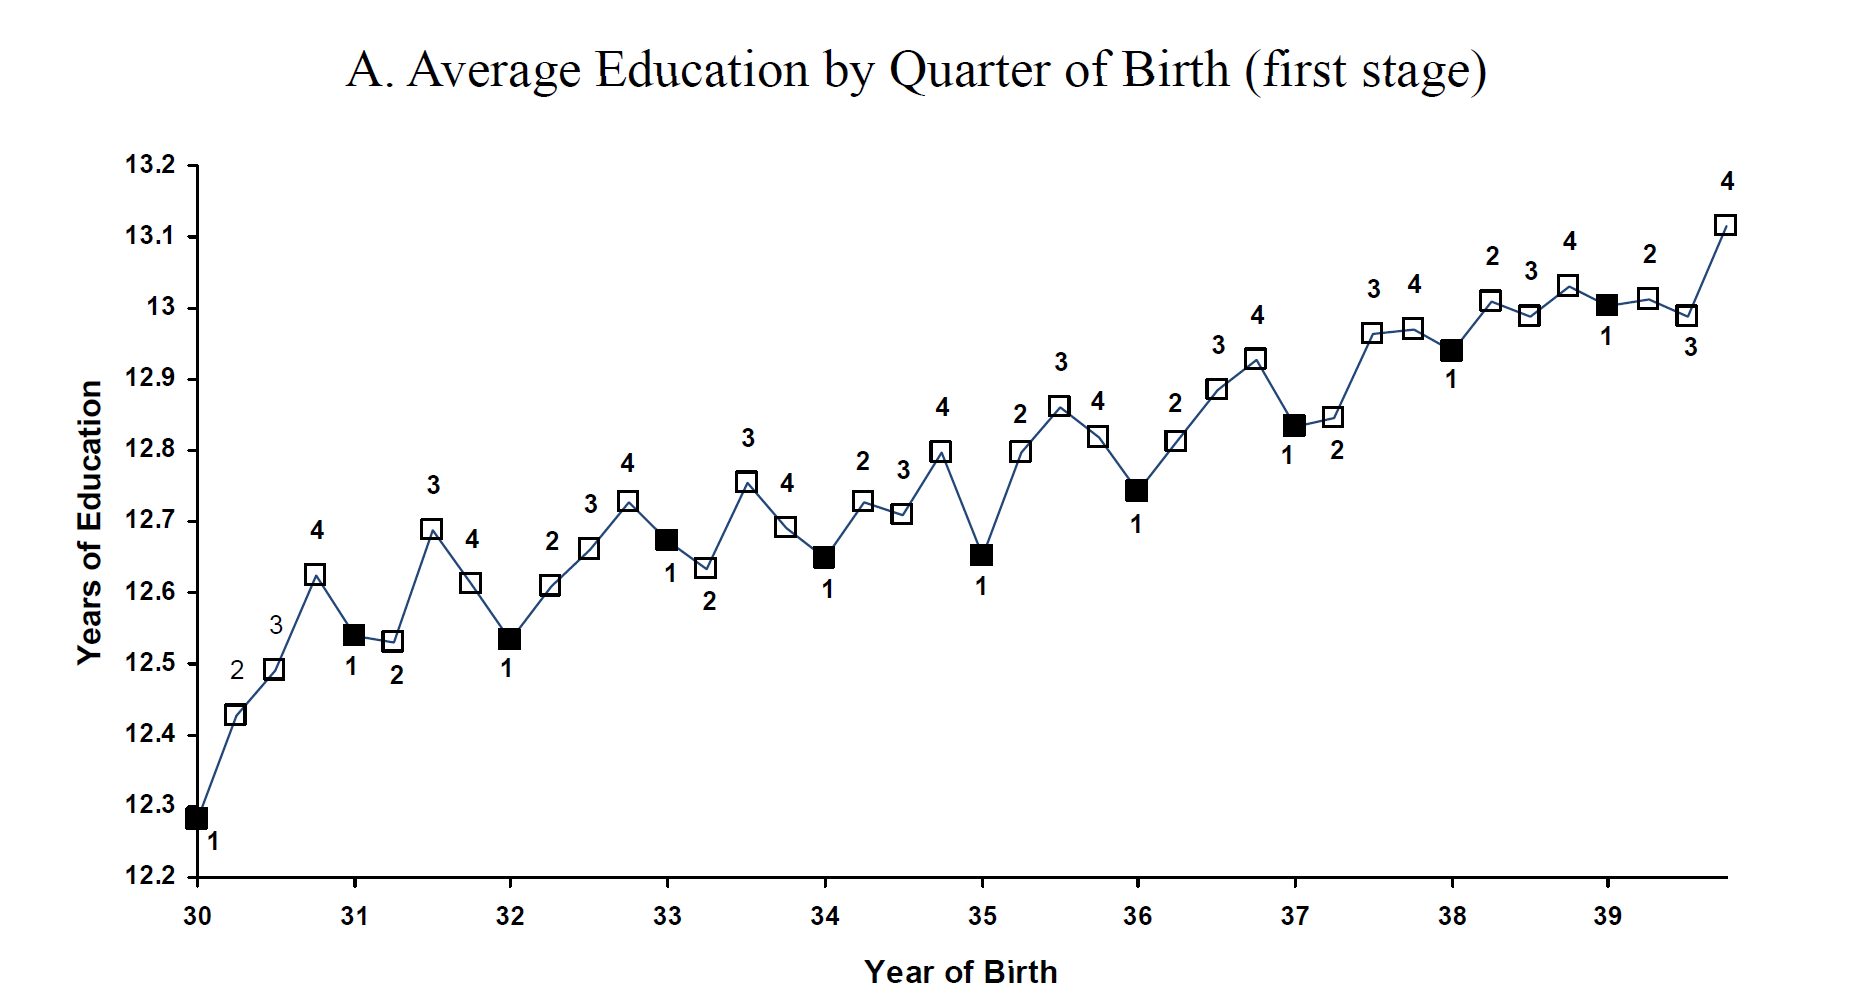
\includegraphics[width=0.8\textwidth]{figures/FirstStageEducQuarterBirth.png}
	\end{figure}
	\end{frame}
	
	\begin{frame}
		\frametitle{Retornos de la educaci\'on (Angrist and Krueger, QJE 1991)}
		\begin{figure}
			\centering
			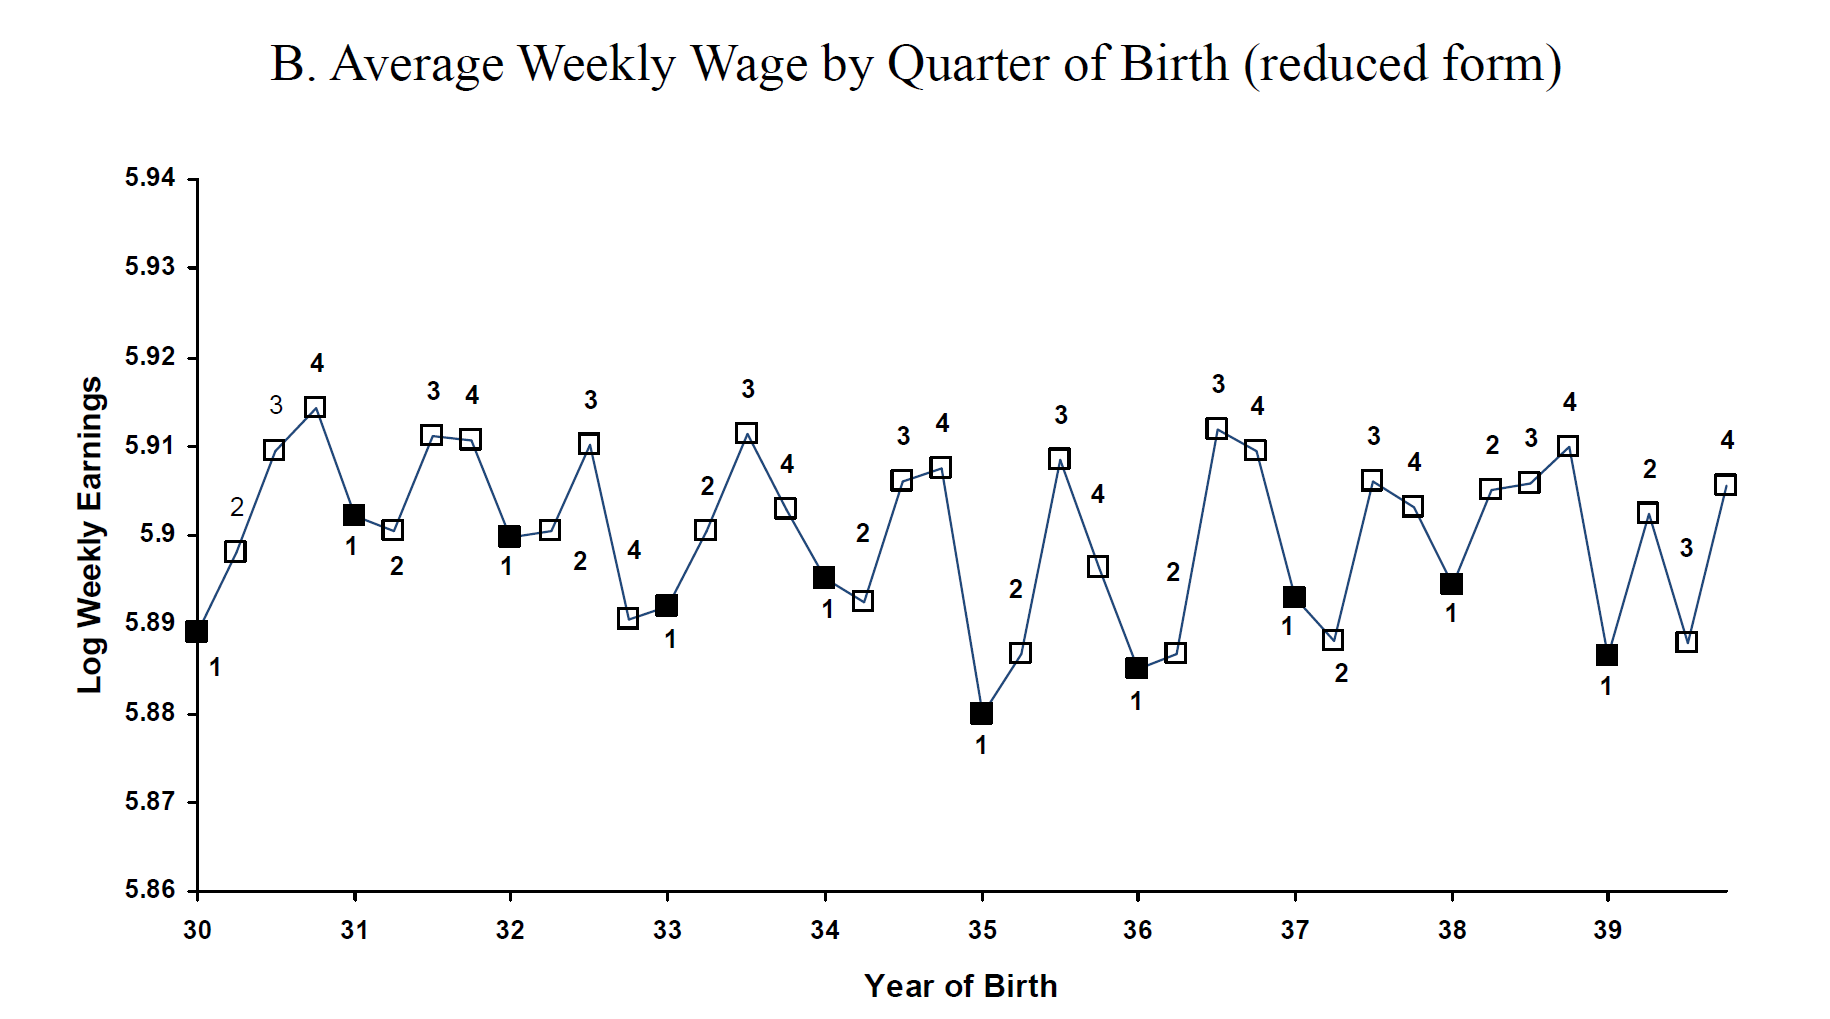
\includegraphics[width=0.8\textwidth]{figures/ReduceFormWageQuarterBirth.png}
		\end{figure}
	\end{frame}

	\begin{frame}
		\frametitle{Retornos de la educaci\'on (Angrist and Krueger, QJE 1991)}
		\begin{figure}
			\centering
			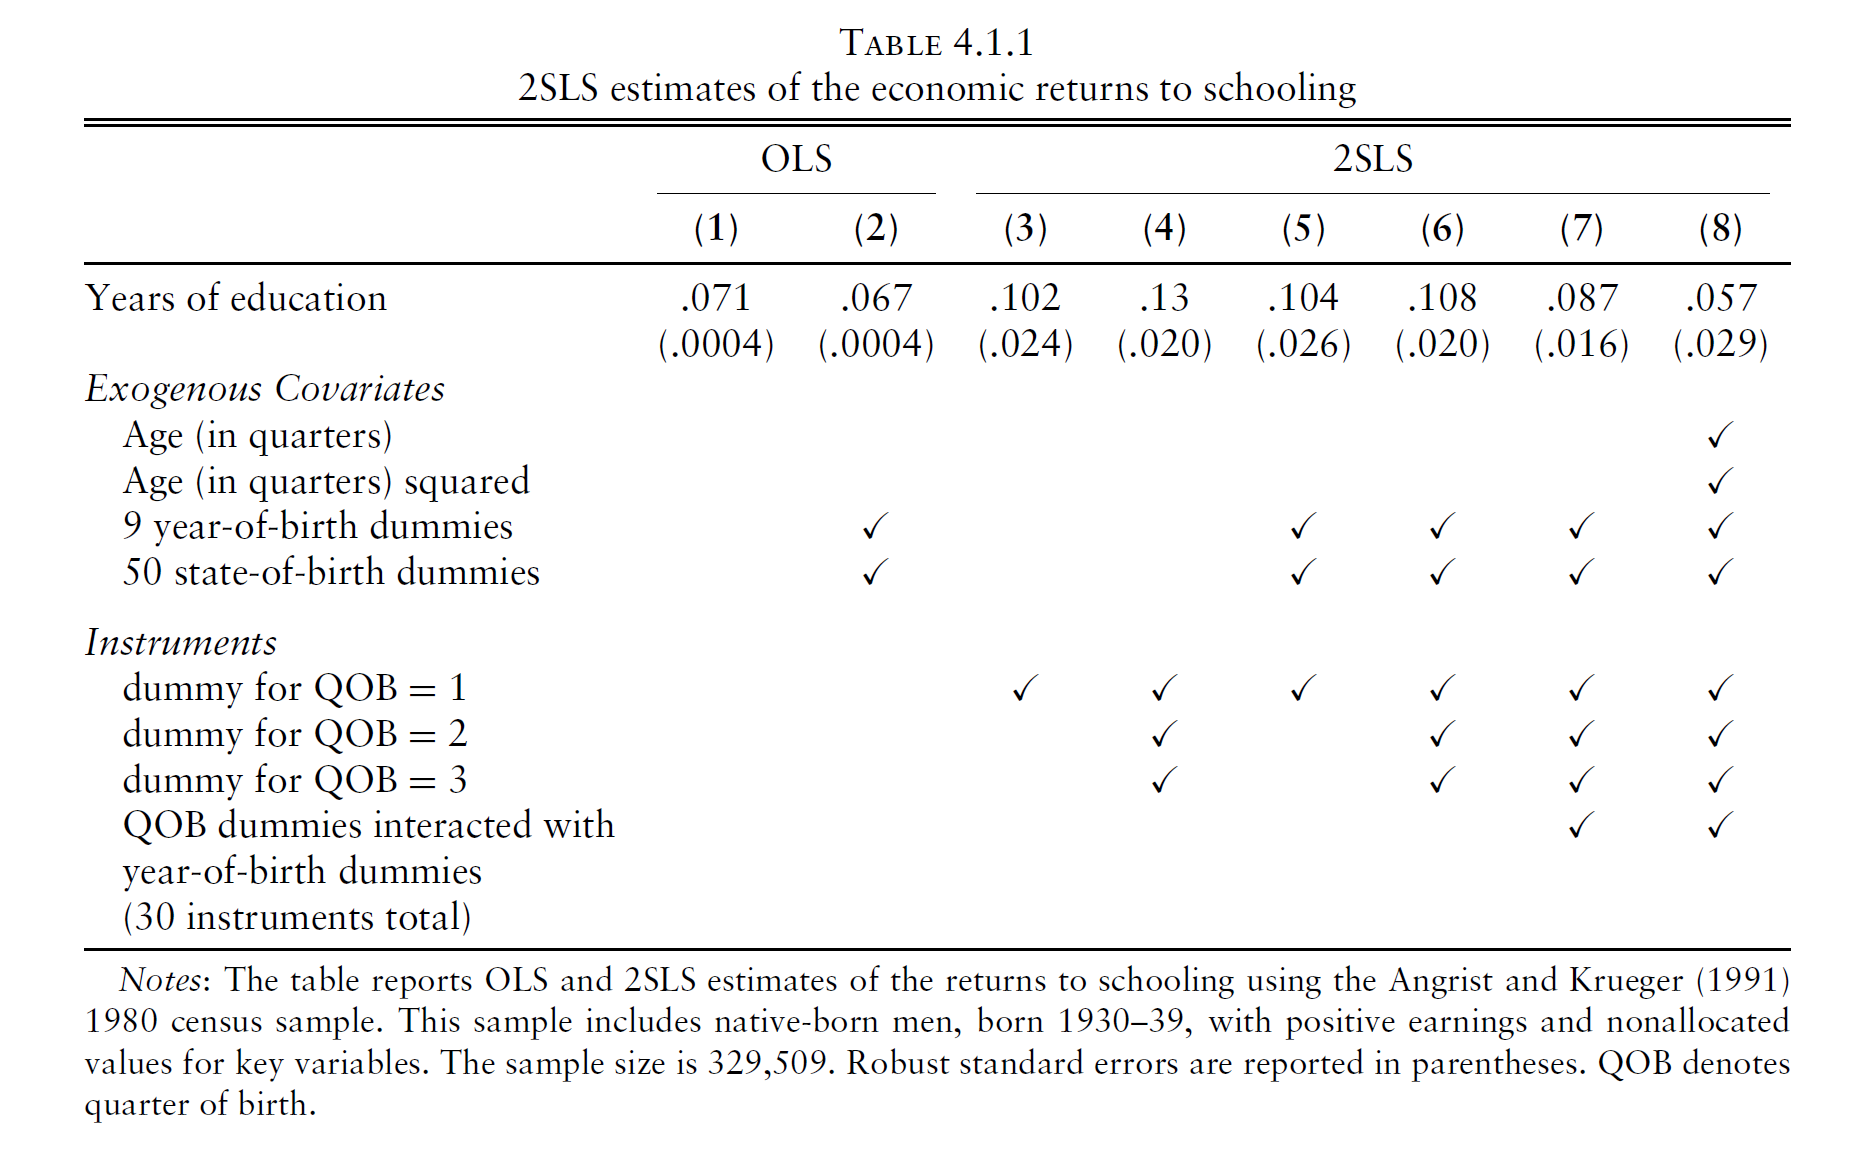
\includegraphics[width=0.8\textwidth]{figures/IVReturnsEducationQuarterBirth.png}
		\end{figure}
	\end{frame}

	\begin{frame}
		\frametitle{Retornos de la educaci\'on (Angrist and Krueger, QJE 1991)}
		\begin{itemize}
			\item Buckles and Hungerman, ``Season of Birth and Later Outcomes: Old Questions, New Answers'' (REStat, 2013).
			\item \alert{Idea}: Ni\~nos nacidos en diferentes meses del a\~no son concebidos por madres con caracter\'isticas sociecon\'omicas diferentes.
			\item Los autores encuentran que ni\~nos nacidos en invierno tienen una mayor probabilidad de haber nacido de una madre adolescente, menor probabilidad de que la madre est\'e casada o la madre tenga secundario completo.
			\item \alert{Mecanismo}: el clima en verano afecta en forma diferencial los patrones de fertilidad de los distintos grupos sociecon\'omicos.
		\end{itemize}
	\end{frame}
	
		% --------------------------------------------------- Slide --
\subsection{Propiedades}
\begin{frame}
    \frametitle{Propiedades de $\hat \beta_{IV}$}
    \begin{itemize}
        \item  <1->Hasta ahora demostramos, en el modelo de regresi\'on simple con un instrumento, el estimador IV es id\'entico a 2SLS.
        \item  <1-> Adem\'as, el estimador de Wald es un caso particular de IV cuando el instrumento es una variable dummy.
        \item  <2->Dado que los tres estimadores son id\'enticos, analizamos las propiedades del estimador IV:
        \begin{align*}
            \hat \beta_{1,IV} =\frac{\widehat{\Cov}(z_i,y_i)}{\widehat{\Cov}(z_i,x_i)},
        \end{align*}
        bajos los supuestos de
    \begin{enumerate}
        \item [IV1]  Muestra aleatoria de tama\~no $N$ $\implies \{y_i,x_i,z_i\}_{i=1}^N$ i.i.d.,
        \item [IV2]  Exogeneidad del instrumento: $\Cov(z_i,u_i)=0$,
        \item [IV3]  Relevancia del instrumento: $\Cov(z_i,x_i)\neq 0$
    \end{enumerate}
        \end{itemize}
\end{frame}

%% --------------------------------------------------- Slide --
%
%\begin{frame}
%    \frametitle{Consistencia}
%\end{frame}
%% --------------------------------------------------- Slide --
%\begin{frame}
%    \frametitle{Consistencia}
%\end{frame}
%\begin{frame}
%    \frametitle{Consistencia}
%\end{frame}

% --------------------------------------------------- Slide --

\begin{frame}
    \frametitle{Consistencia}
        \begin{align*}
            \hat \beta_{1,IV} &=\frac{\widehat{\Cov}(z_i,y_i)}{\widehat{\Cov}(z_i,x_i)}= \frac{\widehat{\Cov}(z_i,\beta_0+\beta_1 x_i+u_i)}{\widehat{\Cov}(z_i,x_i)},\\
            & = \beta_1+\frac{\widehat{\Cov}(z_i,u_i)}{\widehat{\Cov}(z_i,x_i)},
        \end{align*}
        usando los resultados derivados en el cap\'itulo de Teor\'ia asint\'otica, y IV2 (exogeneidad) y IV3 (relevancia)
        \begin{align*}
            \plim \widehat{\Cov}(z_i,x_i) & = {\Cov}(z_i,x_i) \neq 0, \\
            \plim \widehat{\Cov}(z_i,u_i) & = {\Cov}(z_i,u_i) = 0.
        \end{align*}
        Entonces    $\plim \hat \beta_{1,IV}=\beta_{1}$.
\end{frame}

% --------------------------------------------------- Slide --
\begin{frame}
	\frametitle{Discusi\'on: $\hat \beta_{1,IV}$ no es insesgado.}
	\begin{figure}[h!]
		\centering
		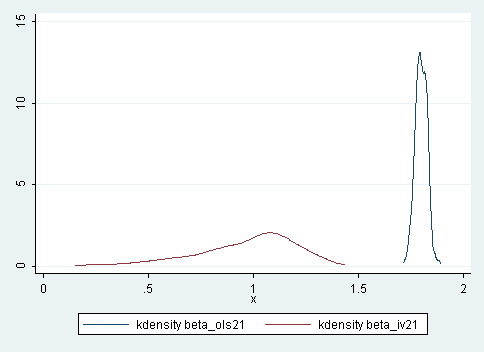
\includegraphics[width=0.45\textwidth]{figures/density_ols_iv2.png}
		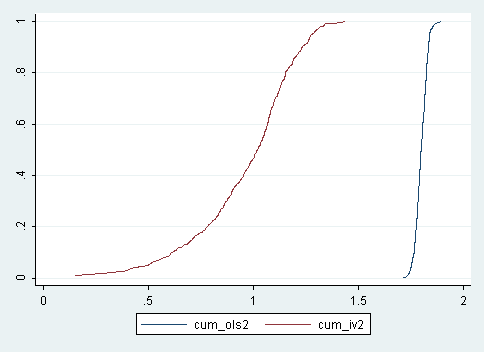
\includegraphics[width=0.45\textwidth]{figures/cdf_ols_iv2.png}
	\end{figure}
	$\beta_1 = 1$ y $N=500$.
\end{frame}
%% --------------------------------------------------- Slide --
%\begin{frame}
%    \frametitle{Distribuci\'on asint\'otica normal}
%\end{frame}
%% --------------------------------------------------- Slide --
%\begin{frame}
%    \frametitle{Distribuci\'on asint\'otica normal}
%\end{frame}
%
%% --------------------------------------------------- Slide --
%\begin{frame}
%    \frametitle{Distribuci\'on asint\'otica normal}
%\end{frame}
%
%% --------------------------------------------------- Slide --
%\begin{frame}
%    \frametitle{Distribuci\'on asint\'otica normal}
%\end{frame}
%
%% --------------------------------------------------- Slide --
%\begin{frame}
%    \frametitle{Distribuci\'on asint\'otica normal}
%\end{frame}
%
%% --------------------------------------------------- Slide --
%\begin{frame}
%    \frametitle{Distribuci\'on asint\'otica normal}
%\end{frame}

% --------------------------------------------------- Slide --
\begin{frame}
    \frametitle{Distribuci\'on asint\'otica normal}
        \begin{align*}
            \sqrt{N} (\hat \beta_{1,IV} - \beta_1)&= \frac{1}{\widehat{\Cov}(z_i,x_i)}\sqrt{N}\widehat{\Cov}(z_i,u_i).
        \end{align*}
        Usando los resultados derivados en el cap\'itulo de Teor\'ia asint\'otica, y IV2 y IV3,
        \begin{align*}
            \plim \widehat{\Cov}(z_i,x_i) & = {\Cov}(z_i,x_i) \neq 0, \\
            \sqrt{N}\widehat{\Cov}(z_i,u_i) &\dto \N (0,V).
        \end{align*}
        donde 
        \begin{align*}
            V&=\E[(z-\E z)^2u^2]-\E[(z-\E z)u]^2,\\
            &=\E[(z-\E z)^2u^2]-\Cov(z,u)^2,\\
            &=\E[(z-\E z)^2u^2].
        \end{align*}
\end{frame}
% --------------------------------------------------- Slide --
\begin{frame}
    \frametitle{Distribuci\'on asint\'otica normal}
    \begin{itemize}
        \item [] Usando el teorema de Slutsky
        \begin{align*}
            \sqrt{N}(\hat \beta_{1,IV} - \beta_1) &\dto \N \left(0,\frac{\E[(z-\E z)^2u^2]}{\Cov(z,x)^2}\right).
        \end{align*}
        \item  \alert{Solamente} para obtener intuici\'on y comparar con MCO asumimos homoscedasticidad ($\E(u^2|z)=\E(u^2)=\sigma^2$) y obtenemos:
        \item [] 
        \begin{align*}
        	V&=\E[(z-\E z)^2u^2]=\Var(z)\E(u^2).
        \end{align*}
        \item [] 
        \begin{align*}
            \sqrt{N}(\hat \beta_{1,IV} - \beta_1) &\dto \N \left(0,\frac{\Var(z)\sigma^2}{\Cov(z,x)^2}\right),\\
            &\dto \N \left(0,\frac{\sigma^2}{\rho_{x,z}^2\Var(x)}\right).
        \end{align*}
    \end{itemize}
\end{frame}
% --------------------------------------------------- Slide --
\begin{frame}
    \frametitle{Distribuci\'on asint\'otica normal}
    \begin{itemize}
        \item  Decimos
                \begin{align*}
                    &\hat \beta_{1,IV} \adistr \N(\beta,\Avar(\hat\beta_{1,IV})),\text{ donde}\\
                    &\Avar(\hat \beta_{1,IV})=\frac{1}{N}\frac{\sigma^2}{\rho_{x,z}^2\Var(x)}.
                \end{align*}
    \end{itemize}
\end{frame}

% --------------------------------------------------- Slide --
\begin{frame}
    \frametitle{Distribuci\'on asint\'otica normal}
            \begin{align*}
            \Avar(\hat \beta_{1,OLS})&=\frac{\sigma^2}{N}\frac{1}{\Var(x)},\\
            \Avar(\hat \beta_{1,IV})&=\frac{\sigma^2}{N}\frac{1}{\rho_{x,z}^2\Var(x)}.
            \end{align*}
\end{frame}

	% --------------------------------------------------- Slide --
    \begin{frame}  [fragile=singleslide]
        \frametitle{Efecto de la fertilidad en la oferta laboral (Angrist y Evans, AER 1998)}
	Estimaci\'on MCO
	\tiny
	\begin{verbatim}
	.          reg hourswm morekids, robust
	
	Linear regression                                      Number of obs =  262793
	                                                       F(  1,262791) = 2540.58
	                                                       Prob > F      =  0.0000
	                                                       R-squared     =  0.0095
	                                                       Root MSE      =  18.287
	
	------------------------------------------------------------------------------
	             |               Robust
	     hourswm |      Coef.   Std. Err.      t    P>|t|     [95% Conf. Interval]
	-------------+----------------------------------------------------------------
	    morekids |  -3.687237   .0731534   -50.40   0.000    -3.830616   -3.543858
	       _cons |   18.23282   .0456501   399.40   0.000     18.14335    18.32229
	------------------------------------------------------------------------------
	\end{verbatim}
\end{frame}
% --------------------------------------------------- Slide --
\begin{frame}  [fragile=singleslide]
	\frametitle{M\'inimos cuadrados en 2 etapas}
	\tiny
		\begin{verbatim}
		.    ivregress 2sls hourswm (morekids = samesex), robust
		
		Instrumental variables (2SLS) regression               Number of obs =  262793
		                                                       Wald chi2(1)  =   25.74
		                                                       Prob > chi2   =  0.0000
		                                                       R-squared     =  0.0074
		                                                       Root MSE      =  18.306
		
		------------------------------------------------------------------------------
		             |               Robust
		     hourswm |      Coef.   Std. Err.      z    P>|z|     [95% Conf. Interval]
		-------------+----------------------------------------------------------------
		    morekids |  -5.409112   1.066216    -5.07   0.000    -7.498856   -3.319368
		       _cons |   18.89348   .4108644    45.98   0.000      18.0882    19.69876
		------------------------------------------------------------------------------
		Instrumented:  morekids
		Instruments:   samesex
		\end{verbatim}
\end{frame}
%% --------------------------------------------------- Slide --
%\subsection{Discusi\'on}
%\begin{frame}
%	\frametitle{Estimador 2SLS a mano}
%	\begin{itemize}
%		\item  Si calculamos el estimador por $2SLS$ ``a mano'' haciendo 2 regresiones MCO, los errores est\'andar est\'an mal calculados. Stata estima $\sigma^2$ usando $\tilde u_i=y_i-\hat \beta_0-\hat \beta_1 \hat x_i$ en lugar de $\hat u_i=y_i-\hat \beta_0-\hat \beta_1 x_i$.
%	\end{itemize}
%\end{frame}
%	% --------------------------------------------------- Slide --
%	\begin{frame}   [fragile=singleslide]
%		\frametitle{Efecto de la fertilidad en la oferta laboral (Angrist y Evans, AER 1998)}
%
%		M\'inimos cuadrados en 2 etapas: A mano
%		\tiny{
%			\begin{verbatim}
%			.          reg hourswm morekidshat, robust
%			
%			Linear regression                                      Number of obs =  262793
%			                                                       F(  1,262791) =   25.55
%			                                                       Prob > F      =  0.0000
%			                                                       R-squared     =  0.0001
%			                                                       Root MSE      =  18.374
%			
%			------------------------------------------------------------------------------
%			             |               Robust
%			     hourswm |      Coef.   Std. Err.      t    P>|t|     [95% Conf. Interval]
%			-------------+----------------------------------------------------------------
%			 morekidshat |  -5.409112   1.070149    -5.05   0.000    -7.506575   -3.311649
%			       _cons |   18.89348   .4123485    45.82   0.000     18.08529    19.70167
%			------------------------------------------------------------------------------
%			
%			\end{verbatim}
%		}
%	\end{frame}
%	
%	% --------------------------------------------------- Slide --
%	\begin{frame}  [fragile=singleslide]
%		\frametitle{M\'inimos cuadrados en 2 etapas}
%		\tiny{
%			\begin{verbatim}
%			.    ivregress 2sls hourswm (morekids = samesex), robust
%			
%			Instrumental variables (2SLS) regression               Number of obs =  262793
%			                                                       Wald chi2(1)  =   25.74
%			                                                       Prob > chi2   =  0.0000
%			                                                       R-squared     =  0.0074
%			                                                       Root MSE      =  18.306
%			
%			------------------------------------------------------------------------------
%			             |               Robust
%			     hourswm |      Coef.   Std. Err.      z    P>|z|     [95% Conf. Interval]
%			-------------+----------------------------------------------------------------
%			    morekids |  -5.409112   1.066216    -5.07   0.000    -7.498856   -3.319368
%			       _cons |   18.89348   .4108644    45.98   0.000      18.0882    19.69876
%			------------------------------------------------------------------------------
%			Instrumented:  morekids
%			Instruments:   samesex
%			\end{verbatim}
%		}
%	\end{frame}
%% --------------------------------------------------- Slide --
%\begin{frame}
%	\frametitle{Con controles adicionales tambi\'en se cumple  $\hat \beta_{1,IV}=\hat \beta_{1,ILS}=\hat \beta_{1,\text{2SLS}}$}
%	\begin{itemize}
%		\item Supongamos un modelo motivado por la ecuaci\'on de Mincer
%		\begin{align*}
%		y_i=\alpha'x_i + \rho s_i+u_i,
%		\end{align*}
%		con un instrumento $z_i$, es decir $\Cov(z,u)=0$ y cumple la condici\'on de relevancia.
%		\item La primera etapa es
%		\begin{align*}
%		s_i=\pi_{10}'x_i + \pi_{11} z_i+\epsilon_{1i},
%		\end{align*}
%		y la forma reducida es
%		\begin{align*}
%		y_i=\pi_{20}'x_i + \pi_{21} z_i+\epsilon_{2i}.
%		\end{align*}
%		\item $\hat \rho_{IV}=\hat \rho_{ILS}=\hat \rho_{2SLS}$ donde $\hat \rho_{ILS}=\hat\pi_{21}/\hat\pi_{11}$ y $\hat \rho_{2SLS}$ utiliza $\hat s_i=\hat\pi_{10}'x_i + \hat\pi_{11} z_i$ en MCO.
%	\end{itemize}
%\end{frame}
%	% --------------------------------------------------- Slide --
%	\begin{frame}
%		\frametitle{Efecto de la fertilidad en la oferta laboral (Angrist y Evans, AER 1998)}
%		\begin{itemize}
%			\item  Modelo
%			\begin{align*}
%				hourswm &= \beta_0 + \beta_1\, agem1 + \beta_2 \,agefstm + \beta_3 \,boy1st + \beta_4 \,boy2nd + \\
%				&+\beta_5 \,blackm + \beta_6 \,hispm + \beta_7 \,othracem + \beta_8  \,morekids+ u_i.
%			\end{align*}
%			donde tener 3 hijos o m\'as ($morekids$),  edad de la madre ($agem1$), edad de la madre cuando tuvo su primer hijo ($agefstm$), primer hijo var\'on ($boy1st$), segundo hijo var\'on ($boy2nd$), raza negra ($blackm$), hispano ($hispm$), otra raza distinto de blanco ($othracem$).
%			\item  Instrumentos: Hijos del mismo sexo ($samesex$).
%		\end{itemize}
%	\end{frame}
%	% --------------------------------------------------- Slide --
%\begin{frame}  [fragile=singleslide]
%	\frametitle{Estad\'isticas descriptivas}
%	\tiny{
%		\begin{verbatim}
%		. sum workedm weeksm1 hourswm morekids samesex agem1 agefstm boy1st boy2nd blackm hispm othracem
%		
%		    Variable |       Obs        Mean    Std. Dev.       Min        Max
%		-------------+--------------------------------------------------------
%		     workedm |    262793    .5301892    .4990887          0          1
%		     weeksm1 |    262793    19.10925    21.88929          0         52
%		     hourswm |    262793    16.81808    18.37502          0         99
%		    morekids |    262793     .383686    .4862838          0          1
%		     samesex |    262793    .5053369    .4999725          0          1
%		-------------+--------------------------------------------------------
%		       agem1 |    262793    30.34861     3.40875         21         35
%		     agefstm |    262793    20.76104    2.930449         15         33
%		      boy1st |    262793    .5142565    .4997977          0          1
%		      boy2nd |    262793    .5128105    .4998368          0          1
%		      blackm |    262793    .0578668    .2334919          0          1
%		-------------+--------------------------------------------------------
%		       hispm |    262793    .0268386    .1616119          0          1
%		    othracem |    262793    .0304422     .171801          0          1
%		
%		\end{verbatim}
%	}
%\end{frame}
%% --------------------------------------------------- Slide --
%\begin{frame}  [fragile=singleslide]
%	\frametitle{Estimaci\'on MCO}
%	\tiny{
%		\begin{verbatim}
%		.     reg hourswm morekids agem1 agefstm boy1st boy2nd blackm hispm othracem, robust
%		
%		Linear regression                                      Number of obs =  262793
%		                                                       F(  8,262784) = 2437.25
%		                                                       Prob > F      =  0.0000
%		                                                       R-squared     =  0.0653
%		                                                       Root MSE      =  17.765
%		
%		------------------------------------------------------------------------------
%		             |               Robust
%		     hourswm |      Coef.   Std. Err.      t    P>|t|     [95% Conf. Interval]
%		-------------+----------------------------------------------------------------
%		    morekids |  -5.957481   .0728214   -81.81   0.000    -6.100209   -5.814753
%		       agem1 |   .8097944   .0114719    70.59   0.000     .7873097    .8322791
%		     agefstm |  -1.300171   .0132689   -97.99   0.000    -1.326177   -1.274164
%		      boy1st |   .0391118   .0693415     0.56   0.573    -.0967958    .1750193
%		      boy2nd |  -.1249087   .0693462    -1.80   0.072    -.2608255     .011008
%		      blackm |   9.630827   .1541127    62.49   0.000      9.32877    9.932884
%		       hispm |   3.015114   .2337557    12.90   0.000     2.556959    3.473269
%		    othracem |   5.103791   .2221084    22.98   0.000     4.668465    5.539117
%		       _cons |   20.77098   .3477798    59.72   0.000     20.08934    21.45262
%		------------------------------------------------------------------------------
%		
%		\end{verbatim}
%	}
%\end{frame}
%% --------------------------------------------------- Slide --
%\begin{frame}  [fragile=singleslide]
%	\frametitle{Primera etapa}
%	\tiny{
%		\begin{verbatim}
%		.     reg morekids samesex agem1 agefstm boy1st boy2nd blackm hispm othracem, robust
%		
%		Linear regression                                      Number of obs =  262793
%		                                                       F(  8,262784) = 3192.69
%		                                                       Prob > F      =  0.0000
%		                                                       R-squared     =  0.0794
%		                                                       Root MSE      =  .46659
%		
%		------------------------------------------------------------------------------
%		             |               Robust
%		    morekids |      Coef.   Std. Err.      t    P>|t|     [95% Conf. Interval]
%		-------------+----------------------------------------------------------------
%		     samesex |   .0689516   .0018212    37.86   0.000      .065382    .0725212
%		       agem1 |   .0302071   .0002879   104.91   0.000     .0296427    .0307714
%		     agefstm |  -.0440882   .0003225  -136.72   0.000    -.0447203   -.0434562
%		      boy1st |  -.0108067   .0018215    -5.93   0.000    -.0143767   -.0072366
%		      boy2nd |  -.0107066   .0018215    -5.88   0.000    -.0142767   -.0071366
%		      blackm |   .0686171   .0039888    17.20   0.000     .0607992    .0764351
%		       hispm |   .1655712   .0056546    29.28   0.000     .1544884     .176654
%		    othracem |   .0615884   .0052676    11.69   0.000      .051264    .0719127
%		       _cons |   .3481758   .0088585    39.30   0.000     .3308134    .3655382
%		------------------------------------------------------------------------------
%		
%		
%		\end{verbatim}
%	}
%\end{frame}
%% --------------------------------------------------- Slide --
%\begin{frame}  [fragile=singleslide]
%	\frametitle{Forma reducida}
%	\tiny{
%		\begin{verbatim}
%		.     reg hourswm samesex agem1 agefstm boy1st boy2nd blackm hispm othracem, robust
%		
%		Linear regression                                      Number of obs =  262793
%		                                                       F(  8,262784) = 1455.90
%		                                                       Prob > F      =  0.0000
%		                                                       R-squared     =  0.0423
%		                                                       Root MSE      =  17.982
%		
%		------------------------------------------------------------------------------
%		             |               Robust
%		     hourswm |      Coef.   Std. Err.      t    P>|t|     [95% Conf. Interval]
%		-------------+----------------------------------------------------------------
%		     samesex |  -.3194128     .07021    -4.55   0.000    -.4570225    -.181803
%		       agem1 |   .6299018   .0114271    55.12   0.000     .6075049    .6522987
%		     agefstm |  -1.037585   .0130847   -79.30   0.000    -1.063231   -1.011939
%		      boy1st |    .101202   .0702054     1.44   0.149    -.0363988    .2388027
%		      boy2nd |  -.0636823   .0702058    -0.91   0.364    -.2012838    .0739192
%		      blackm |    9.22257   .1561482    59.06   0.000     8.916523    9.528616
%		       hispm |    2.02869   .2368864     8.56   0.000     1.564399    2.492981
%		    othracem |   4.737459   .2242792    21.12   0.000     4.297877     5.17704
%		       _cons |   18.65245   .3517275    53.03   0.000     17.96307    19.34182
%		------------------------------------------------------------------------------
%		
%		M\'inimos cuadrados indirectos: -.3194128/.0689516 =-4.63242
%		
%		\end{verbatim}
%	}
%\end{frame}
%% --------------------------------------------------- Slide --
%\begin{frame}  [fragile=singleslide]
%	\frametitle{M\'inimos cuadrados en 2 etapas: A mano}
%	\tiny{
%		\begin{verbatim}
%		.     reg hourswm morekidshat2 agem1 agefstm boy1st boy2nd blackm hispm othracem, robust
%		
%		Linear regression                                      Number of obs =  262793
%		                                                       F(  8,262784) = 1455.90
%		                                                       Prob > F      =  0.0000
%		                                                       R-squared     =  0.0423
%		                                                       Root MSE      =  17.982
%		
%		------------------------------------------------------------------------------
%		             |               Robust
%		     hourswm |      Coef.   Std. Err.      t    P>|t|     [95% Conf. Interval]
%		-------------+----------------------------------------------------------------
%		morekidshat2 |  -4.632419   1.018251    -4.55   0.000    -6.628163   -2.636675
%		       agem1 |   .7698337   .0327366    23.52   0.000     .7056707    .8339966
%		     agefstm |   -1.24182   .0466522   -26.62   0.000    -1.333257   -1.150383
%		      boy1st |    .051141   .0707772     0.72   0.470    -.0875803    .1898624
%		      boy2nd |  -.1132798   .0707957    -1.60   0.110    -.2520375    .0254779
%		      blackm |   9.540433   .1706658    55.90   0.000     9.205933    9.874933
%		       hispm |   2.795685   .2905278     9.62   0.000     2.226258    3.365112
%		    othracem |   5.022762   .2326466    21.59   0.000     4.566781    5.478743
%		       _cons |   20.26534   .5230173    38.75   0.000     19.24024    21.29044
%		------------------------------------------------------------------------------
%		
%		
%		\end{verbatim}
%	}
%\end{frame}
%
%% --------------------------------------------------- Slide --
%\begin{frame}  [fragile=singleslide]
%	\frametitle{M\'inimos cuadrados en 2 etapas}
%	\tiny{
%		\begin{verbatim}
%		.     ivregress 2sls hourswm (morekids = samesex) agem1 agefstm boy1st boy2nd blackm hispm othracem, robu
%		> st   
%		
%		Instrumental variables (2SLS) regression               Number of obs =  262793
%		                                                       Wald chi2(8)  =11849.95
%		                                                       Prob > chi2   =  0.0000
%		                                                       R-squared     =  0.0641
%		                                                       Root MSE      =  17.776
%		
%		------------------------------------------------------------------------------
%		             |               Robust
%		     hourswm |      Coef.   Std. Err.      z    P>|z|     [95% Conf. Interval]
%		-------------+----------------------------------------------------------------
%		    morekids |  -4.632419   1.006622    -4.60   0.000    -6.605363   -2.659476
%		       agem1 |   .7698337   .0323659    23.79   0.000     .7063976    .8332697
%		     agefstm |   -1.24182   .0461269   -26.92   0.000    -1.332227   -1.151413
%		      boy1st |    .051141   .0699597     0.73   0.465    -.0859775    .1882595
%		      boy2nd |  -.1132798   .0699865    -1.62   0.106    -.2504508    .0238912
%		      blackm |   9.540433   .1686319    56.58   0.000      9.20992    9.870946
%		       hispm |   2.795685   .2868816     9.75   0.000     2.233407    3.357963
%		    othracem |   5.022762   .2304716    21.79   0.000     4.571046    5.474478
%		       _cons |   20.26534   .5174611    39.16   0.000     19.25114    21.27955
%		------------------------------------------------------------------------------
%		Instrumented:  morekids
%		Instruments:   agem1 agefstm boy1st boy2nd blackm hispm othracem samesex		
%		\end{verbatim}
%	}
%\end{frame}
\subsection{Instrumentos d\'ebiles}
% --------------------------------------------------- Slide --
\begin{frame}
	\frametitle{Instrumentos d\'ebiles}
    \begin{itemize}
        \item  \alert{Instrumentos d\'ebiles}: los instrumentos explican poco de la variabilidad de la variable end\'ogena.
        \item \alert{?`Por qu\'e es un problema?}
        \begin{itemize}
            \item Si el instrumento tiene alguna correlaci\'on con el inobservado, el sesgo asint\'otico de IV puede ser mayor a MCO.
            \item Aumentan los errores est\'andar de la estimaci\'on.
            \item Aproximaci\'on normal es una pobre aproximaci\'on y el sesgo del estimador IV (para un tama\~no de muestra)  aumenta con el n\'umero de instrumentos
        \end{itemize}
    \end{itemize}
    \end{frame}
% --------------------------------------------------- Slide --
\begin{frame}
    \frametitle{Instrumentos d\'ebiles}
    \begin{itemize}
        \item \alert{?`Cuando es un problema?}
        \begin{itemize}
            \item Regla pr\'actica cuando tenemos una variable end\'ogena: Necesitamos un $F_N >10$ en la primera etapa en el test sobre los instrumentos (Stock and Yogo).
        \end{itemize}
%        \item \alert{?`Que hacemos en caso de tener instrumentos d\'ebiles?}
%        \begin{itemize}
%            \item Si tenemos instrumentos fuertes y d\'ebiles, descartar los d\'ebiles.
%            \item Buscar nuevos instrumentos.
%            \item Utilizar m\'etodos menos sensibles a la presencia de instrumentos d\'ebiles como LIML (Limited information maximun likelihood)
%        \end{itemize}
    \end{itemize}
\end{frame}
% --------------------------------------------------- Slide --
\begin{frame}
    \frametitle{Instrumentos d\'ebiles}
\alert{Recomendaciones}
    \begin{itemize}
            \item Reportar la primera etapa y evaluar si los signos son los esperados.
            \item Reportar estad\'istico $F$ sobre los instrumentos en la primera etapa. Criterio F $>$10.
            \item Elegir mejor instrumento y estimar el modelo con un s\'olo instrumento.
            \item Estimar el modelo con todos los instrumentos con LIML.
            \item Comparar los resultados de 2SLS, 2SLS con un instrumento y LIML.
    \end{itemize}
\end{frame}
% --------------------------------------------------- Slide --
\begin{frame}
    \frametitle{Sesgo asint\'otico cuando el instrumento no es ex\'ogeno.}
\end{frame}

\begin{frame}
    \frametitle{Sesgo asint\'otico cuando el instrumento no es ex\'ogeno.}
            \begin{align*}
            \plim \hat \beta_{1,OLS} &= \beta_1+\frac{\sigma_u}{\sigma_x}\rho_{x,u},\\
            \plim \hat \beta_{1,IV} &= \beta_1+\frac{\sigma_u}{\sigma_x}\frac{\rho_{z,u}}{\rho_{z,x}},\\
            sesgo(\hat \beta_{1,IV}) &\leq sesgo(\hat \beta_{1,OLS}),\\
            \iff \frac{\rho_{z,u}}{\rho_{z,x}}& \leq \rho_{x,u}. 
            \end{align*}
\end{frame}

%\begin{frame}
%    \frametitle{Sesgo asint\'otico cuando el instrumento no es ex\'ogeno.}
%\end{frame}


\begin{frame}
	\frametitle{Sesgo asint\'otico cuando el instrumento no es ex\'ogeno.}
    \begin{itemize}
    	\item  Modelo generador de datos
    	\begin{align*}
    	y_i = 1+ x_i+u_i,
    	\end{align*}
    	y tenemos un instrumento disponible $z_i$ tal que
    	\begin{align*}
    	\begin{pmatrix}
    	u \\
    	z \\
    	x
    	\end{pmatrix}
    	=\N
    	\left(
    	0,
    	\begin{pmatrix}
    	1,\rho_{u,z},\rho_{u,x} \\
    	\rho_{u,z},1,\rho_{z,x} \\
    	\rho_{u,x},\rho_{z,x},1
    	\end{pmatrix}
    	\right)
    	\end{align*}
    	\item Tenemos un muestra aleatoria de tama\~no $N=500$, $\{y_i, x_i,z_i\}_{i=1}^{500}$
    \end{itemize}
\end{frame}
% --------------------------------------------------- Slide --
\begin{frame}
	\frametitle{Sesgo asint\'otico cuando el instrumento no es ex\'ogeno.}
	$x$ end\'ogena con $\rho_{u,x}=0.80$, $z$ end\'ogena con $\rho_{z,u}=0.20$ y $\rho_{z,x}=0.20$
	\begin{figure}[h!]
		\centering
		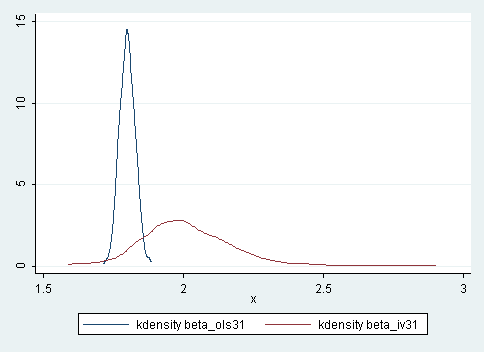
\includegraphics[width=0.45\textwidth]{figures/density_ols_iv3.png}
		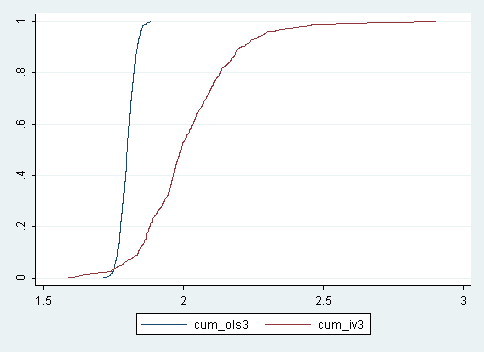
\includegraphics[width=0.45\textwidth]{figures/cdf_ols_iv3.png}
	\end{figure}
	Si el instrumento no es perfecto (est\'a correlado con $u$), el sesgo de IV puede ser mayor al sesgo MCO.
\end{frame}
% --------------------------------------------------- Slide --
\begin{frame}
	\frametitle{Aumentan los errores est\'andar de la estimaci\'on en MCO y IV.}
$x$ ex\'ogena, $z$ ex\'ogena y $\rho_{z,x}=0.20$
	\begin{figure}[h!]
		\centering
		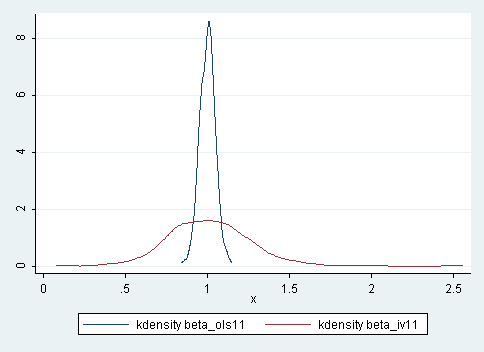
\includegraphics[width=0.45\textwidth]{figures/density_ols_iv1.png}
		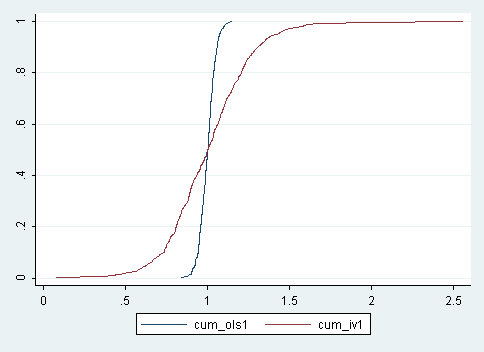
\includegraphics[width=0.45\textwidth]{figures/cdf_ols_iv1.png}
	\end{figure}
    Cuando ambos son consistentes, MCO es m\'as eficiente que IV.
    \end{frame}

% --------------------------------------------------- Slide --
\begin{frame}
	\frametitle{Sesgo del estimador IV  el instrumento es irrelevante}
$x$ end\'ogena con $\rho_{u,x}=0.80$, $z$ ex\'ogena pero irrelevante $\rho_{z,x}=0.00$
  \begin{figure}[h!]
          \centering
          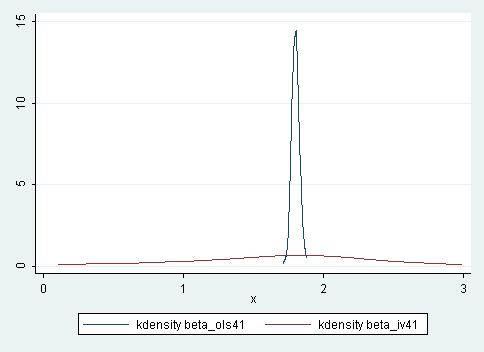
\includegraphics[width=0.45\textwidth]{figures/density_ols_iv4.png}
          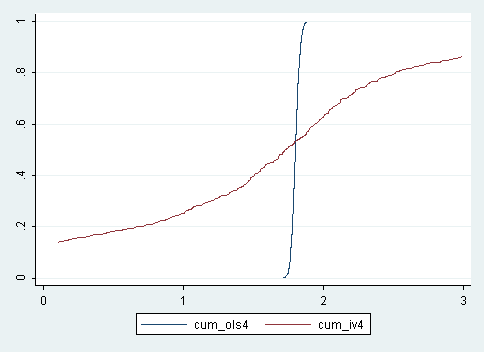
\includegraphics[width=0.45\textwidth]{figures/cdf_ols_iv4.png}
    \end{figure}
    Si el instrumento no cumple la condici\'on de rango, el sesgo  de IV es similar al sesgo de MCO. No es tan grave porque la varianza de la estimaci\'on IV hace que la estimaci\'on no sea informativa.
    \end{frame}
% --------------------------------------------------- Slide --
\begin{frame}
	\frametitle{Sesgo del estimador IV  aumenta con el n\'umero de instrumentos}
    $x$ end\'ogena con $\rho_{u,x}=0.80$, $z$ ex\'ogena y $\rho_{z,x}=0.20$, y  20 instrumentos irrelevantes adicionales
    \begin{figure}[h!]
          \centering
          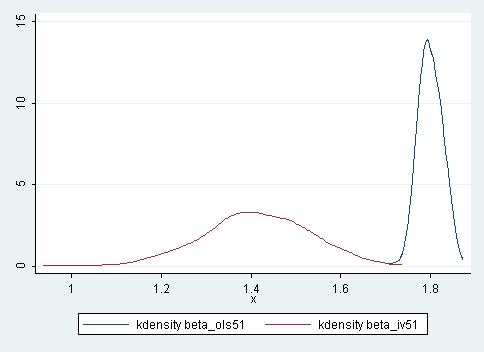
\includegraphics[width=0.45\textwidth]{figures/density_ols_iv5.png}
          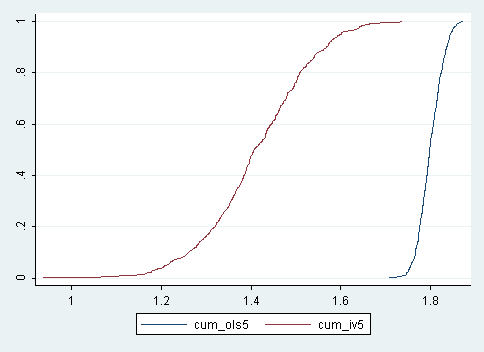
\includegraphics[width=0.45\textwidth]{figures/cdf_ols_iv5.png}
    \end{figure}
    Si tenemos muchos instrumentos d\'ebiles, a medida que aumentan los instrumentos  el sesgo  de IV se acerca al sesgo de MCO. 
\end{frame}


\section{Modelo general}
\begin{frame}
    \frametitle{Modelo general}
    \begin{align*}
        y_i=x_{i}'\beta +u_i,
    \end{align*}
    donde 
    \begin{itemize}
        \item $x_i$ son $K$ \alert{variables explicativas} de donde $K_1$ son \alert{ex\'ogenas} y $K_2$ son \alert{end\'ogenas} ($K=K_1+K_2$), y 
        \item $z_i$ son  $L$ \alert{variables ex\'ogenas} donde $K_1$ son las variables \alert{ex\'ogenas incluidas} en el modelo y $L_1$ son variables \alert{ex\'ogenas excluidas} en el modelo (\alert{instrumentos}) ($L=K_1+L_1$).
    \end{itemize}
    \uncover <2-> {
    Suponemos que $L=dim(z)\geq dim(x)=K \iff L_1\geq K_2$: Tenemos al menos tantos instrumentos como variables end\'ogenas.
   
    Si $L=K$ (y se cumple una condici\'on de rango) el modelo est\'a \alert{exactamente identificado}; si $L>K$ el modelo est\'a potencialmente \alert{sobreidentificado}.
    }
\end{frame}
	% --------------------------------------------------- Slide --
    \begin{frame}
        \frametitle{Efecto de la fertilidad en la oferta laboral (Angrist y Evans)}
  		\begin{itemize}
  		    \small
			\item  \alert{Modelo}
			\begin{align*}
			hourswm &= \beta_0 + \beta_1\, agem1 + \beta_2 \,agefstm + \beta_3 \,boy1st + \beta_4 \,blackm + \\
			&+ \beta_5 \,hispm + \beta_6 \,othracem + \beta_7  \,morekids+ u_i.
			\end{align*}
			donde tener 3 hijos o m\'as ($morekids$),  edad de la madre ($agem1$), edad de la madre cuando tuvo su primer hijo ($agefstm$), primer hijo var\'on ($boy1st$), raza negra ($blackm$), hispano ($hispm$), otra raza distinto de blanco ($othracem$).
			\item \alert{Instrumentos}: Dos hijas mujeres ($girls2$) y dos hijos varones ($boys2$).
			\item <2->Entonces $K=8$, $L=9$.
			
			$x=(1, \, agem1, \,agefstm, \,boy1st, \,blackm, \,hispm, \,othracem, \,morekids )$
			
			$z=(1, \, agem1, \,agefstm, \,boy1st, \,blackm, \,hispm, \,othracem, \,girls2 ,\,boys2 )$
		\end{itemize}
	\end{frame}
% --------------------------------------------------- Slide --
\begin{frame}
    \frametitle{Testear competencia imperfecta en el mercado de pescado de Fulton, NY, Graddy (Rand, 1995)}
    \begin{itemize}
        \item  ?`Es el mercado de pescado de Fulton perfectamente competitivo?
        \item  Evidencia de discriminaci\'on de precios (asi\'aticos pagan precios m\'as bajos).
        \item  Nos enfocamos en la estimaci\'on de la demanda de pescado.
        \item  \alert{Datos}: ventas del d\'ia, precio promedio del d\'ia, d\'ia de la semana y otras variables de un puesto de venta de pescado (merluza) en el mercado de Fulton en Nueva York desde Diciembre de 1991 a Marzo 1992
        
    \end{itemize}
\end{frame}
% --------------------------------------------------- Slide --
\begin{frame}
    \frametitle{Modelo econom\'etrico}
    \begin{itemize}
        \item  []
        \begin{align*}
        ltotqty_t&= \beta_0+\beta_1\, mon_t+\beta_2 \,tues_t+\beta_3\, wed_t+\beta_4 \,thurs_t\\
        &+\alpha \, lavgprc_t +u_t,
        \end{align*}
        donde $lavgprc$: Logaritmo del precio promedio del d\'ia (\$ por libra), $ltotqty$: Logaritmo de ventas totales del d\'ia en libras, $mon$ = 1 para Lunes, $tues$ = 1 para Martes, $wed$ = 1 para Mi\'ercoles, $thurs$ = 1 para Jueves.
        \item \alert{Instrumentos}: $speed2$: M\'inimo en los \'ultimos 2 d\'ias de la velocidad media del viento, $speed3$: M\'inimo hace 3 d\'ias de la velocidad media del viento, $wave2$: M\'aximo en los \'ultimos 2 d\'ias de la altura promedio de las olas, $wave3$: M\'aximo hace 3 y 4 d\'ias de la altura promedio de las olas.
    \end{itemize}
\end{frame}
% --------------------------------------------------- Slide --
\begin{frame}
	\frametitle{Modelo econom\'etrico}
	\begin{itemize}
		\item  []
		\begin{align*}
		ltotqty_t&= \beta_0+\beta_1\, mon_t+\beta_2 \,tues_t+\beta_3\, wed_t+\beta_4 \,thurs_t\\
		&+\alpha \, lavgprc_t +u_t,
		\end{align*}
		\item \alert{Instrumentos}: $speed2$, $speed3$, $wave2$, $wave3$.
		\item <2-> Entonces $K=6$, $L=9$.
		
		$x=(1, \, mon, \,tues, \,wed, \,thurs, \,lavgprc )$
		
		$z=(1, \, mon, \,tues, \,wed, \,thurs, \,speed2, \,speed3, \,wave2, \,wave3 )$
	\end{itemize}
\end{frame}


% --------------------------------------------------- Slide --
\begin{frame}
    \frametitle{Modelo general}
    \begin{align*}
        y_i=x_{i}'\beta +u_i.
    \end{align*}
    Supuestos: $\Cov(x_j,u) \neq 0$ para $j=K_1+1,...,K$.
    \small
    \begin{enumerate}
        \item [IV1]  Muestra aleatoria de tama\~no $N$ $\implies \{y_i,x_i,z_i\}_{i=1}^N$ i.i.d.,
        \bigskip
        \item [IV2]  \alert{Exogeneidad}: $\E(zu)=0$,
        \bigskip
        \item [IV3] \alert{No multicolinealidad perfecta entre ex\'ogenas}: $rango(\E(zz'))=L$
        \bigskip
        \item [IV4] \alert{Condici\'on de rango}: $rango(\E(zx'))=K$.\\
        Una condici\'on necesaria es la \alert{condici\'on de orden}: $L \geq K \iff L_1 \geq K_2$, tenemos tantos instrumentos como variables end\'ogenas.
        \bigskip
       \item [IV5]  $\E(u^2 zz')$ existe.
    \end{enumerate}
\end{frame}
%
%\begin{frame}
%\end{frame}
%
%\begin{frame}
%\end{frame}

% --------------------------------------------------- Slide --
\begin{frame}
    \frametitle{Condici\'on de Rango}
    \begin{itemize} 
        \item La condici\'on $rango(\E(z x'))=K$ es la generalizaci\'on del supuesto de relevancia del modelo simple.
        \item Para \alert{modelo simple} tenemos $x=(1\quad x_1)$ y $z=(1 \quad z_1)$. 
    \end{itemize}
\end{frame}

%\begin{frame}
%    \frametitle{Condici\'on de Rango}
%\end{frame}

% --------------------------------------------------- Slide --
\begin{frame}
    \frametitle{Condici\'on de Rango}
    \begin{itemize} 
        \item La condici\'on $rango(\E(z x'))=K$ es la generalizaci\'on del supuesto de relevancia del modelo simple.
        \item Para \alert{modelo simple} tenemos $x=(1\quad x_1)$ y $z=(1 \quad z_1)$. 
        \item[] Entonces:
        \begin{align*}
        \E(zx')=\left(
        \begin{array}{c c}
        1 & \E(x_1)\\
        \E(z_1) & \E(z_1 x_1)
        \end{array}
        \right).
        \end{align*}
        $rango(\E(zx'))=2$ si y s\'olo s\'i $|\E(zx')|\neq 0$. 
        \item[] <2-> $|\E(zx')|=\E(z_1 x_1)-\E(z_1)\E(x_1)=\Cov(z_1, x_1)\neq 0$.
    \end{itemize}
\end{frame}
% --------------------------------------------------- Slide --
\begin{frame}
	\frametitle{Condici\'on de Rango}
	\begin{itemize} 
		\item  Para \alert{una variable end\'ogena y un instrumento}, la condici\'on de rango es equivalente a contrastar si el instrumento es significativo en la primera etapa.
		\item Para \alert{una variable end\'ogena y m\'ultiples  instrumentos}, la condici\'on de rango es equivalente a contrastar si al menos un instrumento es significativo en la primera etapa.
		\item Para \alert{m\'as de una variable end\'ogena}, una condici\'on suficiente es que instrumentos distintos sean significativos para distintas v. end\'ogenas en la primera etapa. Existen contrastes que eval\'uan si la matriz $\E(zx')$ tiene rango $K$.
		\item  Contraste de Wald (o F) en la primera etapa $H_0:$ los coeficientes de los instrumentos son cero, versus $H_1:$ al menos uno de los coeficientes de los instrumentos es distinto de cero.
	\end{itemize}
\end{frame}
% --------------------------------------------------- Slide --
\subsection{Identificaci\'on y Estimaci\'on}
\begin{frame}
    \frametitle{Identificaci\'on para $L=K$}
    \begin{itemize}
        \item ?`Qu\'e momentos poblacionales permiten identificar los par\'ametros de inter\'es?
        \item [] <2->
        \begin{align*}
        		&\E(z u)=0 \quad \text{usando IV2},\\
        		&\iff \E(z (y-x'\beta)) =0,\\
        		&\iff \E(z y)-\E(z x')\beta =0,\\
        		&\iff \beta=\E(z x')^{-1}\E(z y)\quad \text{usando IV3.b}.
        \end{align*}
        \item  <2-> IV2 y IV3.b son los supuestos que identifican $\beta$.
    \end{itemize}
\end{frame}
% --------------------------------------------------- Slide --
\begin{frame}
    \frametitle{Estimador por variables instrumentales (IV)}
    \begin{itemize}
        \item  Principio de analog\'ia: reemplazar momentos poblacionales por momentos muestrales.
        \item [] <2-> Estamos interesados en:
        \begin{align*}
        		\beta =\E(z x')^{-1}\E(z y).
        \end{align*}
        Usando el principio de analog\'ia, lo estimamos con
        \begin{align*}
        		\hat \beta_{IV} 
        		=\left(
        		\frac{1}{N} \sum z_i x_i'
        		\right)^{-1}\frac{1}{N}\sum z_i y_i .
        \end{align*}
        \item <2-> En notaci\'on matricial: $\hat \beta_{IV}=(Z'X)^{-1}Z'Y$ donde $Z=(z_1,...,z_N)'$.
    \end{itemize}
\end{frame}
% --------------------------------------------------- Slide --
\begin{frame}
	\frametitle{Estimaci\'on para $L \geq K$}
	\small
	\begin{itemize}
		\item Supongamos que tenemos una variable end\'ogena y dos instrumentos: ?`Podemos combinar ambos instrumentos en la estimaci\'on? ?`C\'omo?
		\item <2-> Bajo homoscedasticidad, el mejor instrumento es la combinaci\'on lineal de las variables ex\'ogenas que se obtiene del modelo de regresi\'on de la primera etapa.
		\item <3-> Podemos escribir la primera etapa como
		\begin{align*}
		x=\Pi'z+e,
		\end{align*}
		donde $\Pi: L \times K$ es igual a $\Pi=\E(zz')^{-1}\E(zx')$ y $\E(ze')=0$.
		\item  <3-> El vector de instrumentos de $x$ es:
		\begin{align*}
		x^*=\Pi'z.
		\end{align*}
	   \item <3-> Note que para $x_j$ ex\'ogena usamos la misma variable como instrumento: $x_j^*=x_j$.
	\end{itemize}	
\end{frame}

\begin{frame}
	%\frametitle{Estimaci\'on para $L \geq K$}
	\small
	\begin{itemize}
		\item Podemos escribir la primera etapa como
		\begin{align*}
		x=\Pi'z+e,
		\end{align*}
		donde $\Pi=\E(zz')^{-1}\E(zx')$ y $\E(ze)=0$.
		\item Demostraci\'on:
		\item [] El sistema de ecuaciones de la primera etapa es
		\begin{align*}
		x_1 &= \pi_1'z+e_1,\\
		\vdots\\
		x_K &= \pi_K'z+e_K.
		\end{align*}
		\item [] Se puede escribir
		\begin{align*}
		x = \left[
		\begin{array}{c}
		\pi_1'\\
		\vdots\\
		\pi_K'
		\end{array}
		\right]z+e=[\pi_1 \ldots \pi_K]'z+e=\Pi'z+e.
		\end{align*}
	\end{itemize}
\end{frame}
%
%\begin{frame}
%	\frametitle{Estimaci\'on para $L \geq K$}
%\end{frame}
%
%\begin{frame}
%	\frametitle{Estimaci\'on para $L \geq K$}
%\end{frame}

\begin{frame}
	\frametitle{Estimaci\'on para $L \geq K$}
	\small
	\begin{itemize}
		\item Podemos escribir la primera etapa como
		\begin{align*}
		x=\Pi'z+e,
		\end{align*}
		donde $\Pi=\E(zz')^{-1}\E(zx')$ y $\E(ze')=0$.
		\item Demostraci\'on:
		\item [] El sistema de ecuaciones de la primera etapa es
		\begin{align*}
		x =\Pi'z+e,
		\end{align*}
		donde $\Pi=[\pi_1 \ldots \pi_K]$.
		\item [] Dado que $\pi_j=\E(zz')^{-1}\E(zx_j)$ entonces
		\begin{align*}
		\Pi=[\pi_1 \ldots \pi_K]=\E(zz')^{-1} [\E(zx_1) \ldots \E(zx_K)]=\E(zz')^{-1} \E(zx').
		\end{align*}
	\end{itemize}
\end{frame}

\begin{frame}
	\frametitle{Estimaci\'on para $L \geq K$}
	\small
	\begin{itemize}
		\item Supongamos que tenemos una variable end\'ogena y dos instrumentos: ?`Qu\'e instrumento utilizamos?
		\item Bajo homoscedasticidad, el mejor instrumento es la combinaci\'on lineal de las variables ex\'ogenas que se obtiene del modelo de regresi\'on de la primera etapa.
		\item Podemos escribir la primera etapa como
		\begin{align*}
		x=\Pi'z+e,
		\end{align*}
		donde $\Pi: L \times K$ es igual a $\Pi=\E(zz')^{-1}\E(zx')$ y $\E(ze')=0$.
		\item  El vector de instrumentos de $x$ es:
		\begin{align*}
		x^*=\Pi'z.
		\end{align*}
		\item  Note que para $x_j$ ex\'ogena usamos la misma variable como instrumento: $x_j^*=x_j$.
	\end{itemize}
\end{frame}

% --------------------------------------------------- Slide --
\begin{frame}
    \frametitle{Instrumentos}
	Queremos hacer una estimaci\'on de IV con $x^*=\Pi'z$. Verifiquemos que los instrumentos cumplen la condici\'on de exogeneidad y rango.
\end{frame}

%\begin{frame}
%    \frametitle{Instrumentos}
%\end{frame}
%
%\begin{frame}
%    \frametitle{Instrumentos}
%\end{frame}

\begin{frame}
    \frametitle{Instrumentos}
	Queremos hacer una estimaci\'on de IV con $x^*=\Pi'z$. Verifiquemos que los instrumentos cumplen la condici\'on de exogeneidad y rango.
    \begin{itemize}
    \item \alert{Exogeneidad}
    \item []  $\E(x^*u)=\E(\Pi'zu)=\Pi'\E(zu)=0$ por exogeneidad de $z$.
    \item \alert{Condici\'on de rango}: $rango(\E(x^*x'))=K$.
    \item []  $\E(x^*x')=\E(\Pi'zx')=\Pi'\E(zx')=\E(xz')\E(zz')^{-1}\E(zx')$\\
    Como $rango(\E(zz'))=L$, $rango(\E(zx')=K$ y $L \geq K$ entonces $rango(\E(x^*x'))=K$.
    \end{itemize}
\end{frame}
%% --------------------------------------------------- Slide --
%\begin{frame}
%    \frametitle{Estimaci\'on}
%\end{frame}
%
%\begin{frame}
%    \frametitle{Estimaci\'on}
%\end{frame}
%
%\begin{frame}
%    \frametitle{Estimaci\'on}
%\end{frame}
%
%\begin{frame}
%    \frametitle{Estimaci\'on}
%\end{frame}
%
%\begin{frame}
%    \frametitle{Estimaci\'on}
%\end{frame}
% --------------------------------------------------- Slide --
\begin{frame}
    \frametitle{Estimaci\'on}
    Estimaci\'on en dos etapas:
    \begin{itemize}
    \item Regresar $x_i$ en $z_i$ y obtener valores predichos 
    \begin{align*}
    \hat x_i = \hat\Pi' z_i.
            \end{align*}
    \item [] Nota: Es lo mismo que regresar solamente las variables end\'ogenas y utilizar las variables ex\'ogenas incluidas como su propio instrumento.
    \item Usar $\hat x_i$ como instrumentos en un IV
            \begin{align*}
                \hat \beta_{IV} 
                =\left(
                \frac{1}{N} \sum \hat x_i x_i'
                \right)^{-1}\frac{1}{N}\sum \hat x_i y_i .
            \end{align*}
    \end{itemize}
\end{frame}

\begin{frame}
    \frametitle{Estimaci\'on}
    \begin{itemize}
    \item Dado que $x_i = \hat x_i + \hat e_i$ y de las CPO de MCO
        \begin{align*}
        \frac{1}{N}\sum_i \hat x_i \hat e_i'=0,
        \end{align*}
        entonces
        \begin{align*}
        \frac{1}{N}\sum_i \hat x_i x_i'=\frac{1}{N}\sum_i \hat x_i \hat x_i',
        \end{align*}
        y el estimador IV se puede escribir como un estimador 2SLS
            \begin{align*}
                \hat \beta_{2SLS} 
                =\left(
                \frac{1}{N} \sum \hat x_i \hat x_i'
                \right)^{-1}\frac{1}{N}\sum \hat x_i y_i,
            \end{align*}
            donde la segunda etapa es un regresi\'on de $y$ en $\hat x_i$.
            \item Recuerde: No es recomendable computar el estimador usando el procedimiento en dos etapas porque los s.e. est\'an mal calculados.
    \end{itemize}
\end{frame}
\subsection{Propiedades}
\begin{frame}
    \frametitle{Propiedades}
    \begin{itemize} 
    	\item Para probar consistencia es conveniente escribir el estimador en funci\'on de las variables originales.
    	\item El coeficiente estimado de regresar $x_j$ en los instrumentos es  $\hat \pi_j=\left(\sum z_i z_i'\right)^{-1} \sum z_i x_{ji}$.
    	\item La matriz de dichos coeficientes es $\hat \Pi=[\hat \pi_1 \hat \pi_2 ... \hat \pi_K]=\left(\sum z_i z_i'\right)^{-1} \sum z_i x_{i}'$.
    	\item Por lo tanto podemos escribir:
        \begin{align*}
            \hat \beta_{2SLS} &=\left(
                            \sum \hat x_i \hat x_i'
                            \right)^{-1}\sum \hat x_i y_i,\\
            &=\left[\left(\sum x_i z_i'\right)\left(\sum z_i z_i'\right)^{-1}\left(\sum z_i x_i'\right) \right]^{-1}\\
            &
            \left(\sum x_i z_i'\right)\left(\sum z_i z_i'\right)^{-1}\left(\sum z_i y_i\right).
        \end{align*}
 %       \item En notaci\'on matricial: $\hat \beta_{2SLS}=[(X'Z)(Z'Z)^{-1}(Z'X)]^{-1}(X'Z)(Z'Z)^{-1}(Z'Y)$.
        \item Si $K=L$, tenemos el estimador IV.
    \end{itemize}
\end{frame}

%% --------------------------------------------------- Slide --
%\begin{frame}
%    \frametitle{Consistencia}
%\end{frame}
%\begin{frame}
%    \frametitle{Consistencia}
%\end{frame}

% --------------------------------------------------- Slide --
\begin{frame}
    \frametitle{Consistencia}
        \begin{align*}
            \hat \beta_{2SLS} &=\beta+\left[\left(\sum x_i z_i'\right)\left(\sum z_i z_i'\right)^{-1}\left(\sum z_i x_i'\right) \right]^{-1}\\
                        &
                        \left(\sum x_i z_i'\right)\left(\sum z_i z_i'\right)^{-1}\left(\sum z_i u_i\right)
        \end{align*}
        Entonces usando los resultados derivados en el cap\'itulo de Teor\'ia asint\'otica, y IV2 y IV3
        \begin{align*}
            \plim\hat \beta_{2SLS} &=\beta+[\E(xz')\E(zz')^{-1}\E(zx')]^{-1}\E(xz')\E(zz')^{-1}\E(zu).
        \end{align*}
        Entonces $\plim \hat \beta_{2SLS}=\beta$.
\end{frame}
% --------------------------------------------------- Slide --
%\begin{frame}
%    \frametitle{Distribuci\'on asint\'otica normal}
%\end{frame}
%
%\begin{frame}
%    \frametitle{Distribuci\'on asint\'otica normal}
%\end{frame}
%
%\begin{frame}
%    \frametitle{Distribuci\'on asint\'otica normal}
%\end{frame}

\begin{frame}
    \frametitle{Distribuci\'on asint\'otica normal}
        \begin{align*}
            \sqrt{N} (\hat \beta_{2SLS} - \beta)&= \left[\left(\sum x_i z_i'\right)\left(\sum z_i z_i'\right)^{-1}\left(\sum z_i x_i'\right) \right]^{-1}\\
                                    &
                                    \left(\sum x_i z_i'\right)\left(\sum z_i z_i'\right)^{-1}\sqrt{N} \left(\sum z_i u_i\right)
        \end{align*}
        Usando los resultados derivados en el cap\'itulo de Teor\'ia asint\'otica, y IV2, IV3, y IV4, y el  teorema de Slutsky,
        \begin{align*}
            \sqrt{N} (\hat \beta_{2SLS} - \beta)&\dto \N(0,B^{-1}CB^{-1}),
        \end{align*}
        donde 
        \begin{align*}
            B&=\E(xz')\E(zz')^{-1}\E(zx'),\\
            C&=\E(xz')\E(zz')^{-1}\E(u^2zz') \E(zz')^{-1}\E(zx').
        \end{align*}
\end{frame}
% --------------------------------------------------- Slide --
\begin{frame}
    \frametitle{Distribuci\'on asint\'otica normal}
    \begin{itemize}
        \item  Decimos
                \begin{align*}
                    &\hat \beta_{2SLS} \adistr \N(\beta,\Avar(\hat\beta_{2SLS})),\text{ donde}\\
                    &\Avar(\hat \beta_{2SLS})=\frac{1}{N}B^{-1}CB^{-1}.
                \end{align*}
         \item  Estimaci\'on consistente de $\Avar(\hat \beta_{2SLS})$: Reemplazamos momentos poblacionales por muestrales y errores poblacionales ($u_i$) por errores estimados ($\hat u_i$). Es decir,
                \begin{align*}
                    \widehat{\Avar}(\hat \beta_{2SLS})=\frac{1}{N}\hat B^{-1}\hat C \hat B^{-1},
                \end{align*}
                donde
                \scriptsize
                \begin{align*}
                    \hat B=&\left(\frac{1}{N}\sum x_i z_i'\right)\left(\frac{1}{N}\sum z_i z_i'\right)^{-1}\left(\frac{1}{N}\sum z_i x_i'\right),\\
                    \hat C=&\left(\frac{1}{N}\sum x_i z_i'\right)\left(\frac{1}{N}\sum z_i z_i'\right)^{-1}
                    \left(\frac{1}{N}\sum \hat u_i^2 z_i z_i'\right)
                    \left(\frac{1}{N}\sum z_i z_i'\right)^{-1}\left(\frac{1}{N}\sum z_i x_i'\right).
                \end{align*}
    \end{itemize}
\end{frame}
% --------------------------------------------------- Slide --
\begin{frame}
    \frametitle{Eficiencia}
    \begin{itemize}
        \item  Si asumimos homoscedasticidad, es decir IV5 $\E(u^2|z)=\E(u^2)=\sigma^2$:
                \begin{align*}
                    &\Avar(\hat \beta_{2SLS})=\frac{1}{N}\sigma^2 B^{-1}.
                \end{align*}
    \end{itemize}
\end{frame}
% --------------------------------------------------- Slide --
\begin{frame}
    \frametitle{Efecto de la fertilidad en la oferta laboral (Angrist y Evans, AER 1998)}
    \begin{itemize}
			\item  \alert{Modelo}
			\begin{align*}
			hourswm &= \beta_0 + \beta_1\, agem1 + \beta_2 \,agefstm + \beta_3 \,boy1st + \beta_4 \,blackm + \\
			&+ \beta_5 \,hispm + \beta_6 \,othracem + \beta_7  \,morekids+ u_i.
			\end{align*}
			donde tener 3 hijos o m\'as ($morekids$),  edad de la madre ($agem1$), edad de la madre cuando tuvo su primer hijo ($agefstm$), primer hijo var\'on ($boy1st$), raza negra ($blackm$), hispano ($hispm$), otra raza distinto de blanco ($othracem$).
			\item  \alert{Instrumentos}: Dos hijas mujeres ($girls2$) y dos hijos varones ($boys2$).
    \end{itemize}
\end{frame}
% --------------------------------------------------- Slide --
\begin{frame}  [fragile=singleslide]
    \frametitle{MCO}
    \tiny
    \begin{verbatim}
.     reg hourswm morekids agem1 agefstm boy1st blackm hispm othracem, robust

Linear regression                                      Number of obs =  262793
                                                       F(  7,262785) = 2784.79
                                                       Prob > F      =  0.0000
                                                       R-squared     =  0.0653
                                                       Root MSE      =  17.766

------------------------------------------------------------------------------
             |               Robust
     hourswm |      Coef.   Std. Err.      t    P>|t|     [95% Conf. Interval]
-------------+----------------------------------------------------------------
    morekids |   -5.95623   .0728213   -81.79   0.000    -6.098958   -5.813503
       agem1 |   .8097462    .011472    70.58   0.000     .7872614     .832231
     agefstm |  -1.300151   .0132688   -97.99   0.000    -1.326158   -1.274145
      boy1st |   .0378813   .0693342     0.55   0.585    -.0980118    .1737745
      blackm |   9.631453   .1541123    62.50   0.000     9.329397    9.933509
       hispm |   3.014593   .2337595    12.90   0.000      2.55643    3.472755
    othracem |   5.103861   .2220974    22.98   0.000     4.668556    5.539166
       _cons |   20.70811   .3460431    59.84   0.000     20.02988    21.38635
------------------------------------------------------------------------------
    \end{verbatim}
\end{frame}

% --------------------------------------------------- Slide --
\begin{frame}  [fragile=singleslide]
    \frametitle{Primera etapa}
    \tiny
    \begin{verbatim}
.    * First stage
.     reg morekids boys2 girls2 agem1 agefstm boy1st blackm hispm othracem, robust

Linear regression                                      Number of obs =  262793
                                                       F(  8,262784) = 3192.69
                                                       Prob > F      =  0.0000
                                                       R-squared     =  0.0794
                                                       Root MSE      =  .46659

------------------------------------------------------------------------------
             |               Robust
    morekids |      Coef.   Std. Err.      t    P>|t|     [95% Conf. Interval]
-------------+----------------------------------------------------------------
       boys2 |    .058245   .0025344    22.98   0.000     .0532776    .0632124
      girls2 |   .0796582   .0026165    30.44   0.000       .07453    .0847865
       agem1 |   .0302071   .0002879   104.91   0.000     .0296427    .0307714
     agefstm |  -.0440882   .0003225  -136.72   0.000    -.0447203   -.0434562
       _cons |   .3374692   .0088555    38.11   0.000     .3201126    .3548258
------------------------------------------------------------------------------

.     test  boys2 girls2
 ( 1)  boys2 = 0
 ( 2)  girls2 = 0

       F(  2,262784) =  727.61
            Prob > F =    0.0000

    \end{verbatim}
\end{frame}
%% --------------------------------------------------- Slide --
%\begin{frame}  [fragile=singleslide]
%    \frametitle{Forma reducida}
%    \tiny{
%    \begin{verbatim}
%.    * Reduced form
%.    
%.     reg hourswm  boys2 girls2 agem1 agefstm boy1st blackm hispm othracem, robust
%
%Linear regression                                      Number of obs =  262793
%                                                       F(  8,262784) = 1455.90
%                                                       Prob > F      =  0.0000
%                                                       R-squared     =  0.0423
%                                                       Root MSE      =  17.982
%
%------------------------------------------------------------------------------
%             |               Robust
%     hourswm |      Coef.   Std. Err.      t    P>|t|     [95% Conf. Interval]
%-------------+----------------------------------------------------------------
%       boys2 |   -.383095   .0981251    -3.90   0.000    -.5754175   -.1907725
%      girls2 |  -.2557305   .1004394    -2.55   0.011     -.452589   -.0588719
%       agem1 |   .6299018   .0114271    55.12   0.000     .6075049    .6522987
%     agefstm |  -1.037585   .0130847   -79.30   0.000    -1.063231   -1.011939
%      boy1st |   .1648842   .0999877     1.65   0.099    -.0310889    .3608574
%      blackm |    9.22257   .1561482    59.06   0.000     8.916523    9.528616
%       hispm |    2.02869   .2368864     8.56   0.000     1.564399    2.492981
%    othracem |   4.737459   .2242792    21.12   0.000     4.297877     5.17704
%       _cons |   18.58877   .3518488    52.83   0.000     17.89915    19.27838
%------------------------------------------------------------------------------
%
%
%    \end{verbatim}
%    }
%\end{frame}
\begin{frame}  [fragile=singleslide]
	\frametitle{IV con prediccion de la primera etapa}
	\tiny
		\begin{verbatim}
		ivregress 2sls hourswm (morekids = morekidshat3) agem1 agefstm boy1st blackm hispm othrace
		> m, robust  
		
Instrumental variables (2SLS) regression               Number of obs =  262793
                                                       Wald chi2(7)  =11845.37
                                                       Prob > chi2   =  0.0000
                                                       R-squared     =  0.0637
                                                       Root MSE      =   17.78

------------------------------------------------------------------------------
             |               Robust
     hourswm |      Coef.   Std. Err.      z    P>|z|     [95% Conf. Interval]
-------------+----------------------------------------------------------------
    morekids |  -4.426483   .9981875    -4.43   0.000    -6.382894   -2.470071
       agem1 |   .7636138   .0321289    23.77   0.000     .7006423    .8265852
     agefstm |  -1.232783   .0457746   -26.93   0.000      -1.3225   -1.143067
      boy1st |   .0519022   .0699756     0.74   0.458    -.0852475     .189052
      blackm |    9.52702   .1684359    56.56   0.000     9.196891    9.857148
       hispm |   2.761302   .2861099     9.65   0.000     2.200536    3.322067
    othracem |   5.010299   .2303647    21.75   0.000     4.558793    5.461806
       _cons |   20.13108   .5105939    39.43   0.000     19.13033    21.13182
------------------------------------------------------------------------------
Instrumented:  morekids
Instruments:   agem1 agefstm boy1st blackm hispm othracem morekidshat3
\end{verbatim}
\end{frame}

% --------------------------------------------------- Slide --
\begin{frame}  [fragile=singleslide]
    \frametitle{Dos veces MCO}
    \tiny
    \begin{verbatim}
.     reg hourswm morekidshat3 agem1 agefstm boy1st blackm hispm othracem, robust

Linear regression                                      Number of obs =  262793
                                                       F(  7,262785) = 1663.58
                                                       Prob > F      =  0.0000
                                                       R-squared     =  0.0423
                                                       Root MSE      =  17.982

------------------------------------------------------------------------------
             |               Robust
     hourswm |      Coef.   Std. Err.      t    P>|t|     [95% Conf. Interval]
-------------+----------------------------------------------------------------
morekidshat3 |  -4.426483   1.009505    -4.38   0.000    -6.405085    -2.44788
       agem1 |   .7636138   .0324912    23.50   0.000      .699932    .8272956
     agefstm |  -1.232783   .0462865   -26.63   0.000    -1.323504   -1.142063
      boy1st |   .0519022   .0707778     0.73   0.463    -.0868204    .1906249
      blackm |    9.52702   .1704203    55.90   0.000        9.193    9.861039
       hispm |   2.761302   .2896682     9.53   0.000      2.19356    3.329043
    othracem |   5.010299   .2325027    21.55   0.000       4.5546    5.465998
       _cons |   20.13108   .5159306    39.02   0.000     19.11987    21.14229
------------------------------------------------------------------------------


    \end{verbatim}
\end{frame}

% --------------------------------------------------- Slide --
\begin{frame}  [fragile=singleslide]
    \frametitle{M\'inimos cuadrados en 2 etapas}
    \tiny
    \begin{verbatim}
.     ivregress 2sls hourswm (morekids = boys2 girls2) agem1 agefstm boy1st blackm hispm othracem, robust   

Instrumental variables (2SLS) regression               Number of obs =  262793
                                                       Wald chi2(7)  =11845.37
                                                       Prob > chi2   =  0.0000
                                                       R-squared     =  0.0637
                                                       Root MSE      =   17.78

------------------------------------------------------------------------------
             |               Robust
     hourswm |      Coef.   Std. Err.      z    P>|z|     [95% Conf. Interval]
-------------+----------------------------------------------------------------
    morekids |  -4.426483   .9981875    -4.43   0.000    -6.382894   -2.470071
       agem1 |   .7636138   .0321289    23.77   0.000     .7006423    .8265852
     agefstm |  -1.232783   .0457746   -26.93   0.000      -1.3225   -1.143067
      boy1st |   .0519022   .0699756     0.74   0.458    -.0852475     .189052
      blackm |    9.52702   .1684359    56.56   0.000     9.196891    9.857148
       hispm |   2.761302   .2861099     9.65   0.000     2.200536    3.322067
    othracem |   5.010299   .2303647    21.75   0.000     4.558793    5.461806
       _cons |   20.13108   .5105939    39.43   0.000     19.13033    21.13182
------------------------------------------------------------------------------
Instrumented:  morekids
Instruments:   agem1 agefstm boy1st blackm hispm othracem boys2 girls2

    \end{verbatim}
\end{frame}

%% --------------------------------------------------- Slide --
%\begin{frame}  [fragile=singleslide]
%    \frametitle{Modelo exactamente identificado: girls2}
%    \tiny{
%    \begin{verbatim}
%.     ivregress 2sls hourswm (morekids = girls2) agem1 agefstm boy1st blackm hispm othracem, robust   
%
%Instrumental variables (2SLS) regression               Number of obs =  262793
%                                                       Wald chi2(7)  =11802.34
%                                                       Prob > chi2   =  0.0000
%                                                       R-squared     =  0.0604
%                                                       Root MSE      =  17.812
%
%------------------------------------------------------------------------------
%             |               Robust
%     hourswm |      Coef.   Std. Err.      z    P>|z|     [95% Conf. Interval]
%-------------+----------------------------------------------------------------
%    morekids |  -3.210314   1.248982    -2.57   0.010    -5.658274   -.7623539
%------------------------------------------------------------------------------
%Instrumented:  morekids
%Instruments:   agem1 agefstm boy1st blackm hispm othracem girls2
%
%    \end{verbatim}
%    }
%\end{frame}
%% --------------------------------------------------- Slide --
%\begin{frame}  [fragile=singleslide]
%	\frametitle{Modelo exactamente identificado: boys2}
%	\tiny{
%		\begin{verbatim}
%
%		ivregress 2sls hourswm (morekids = boys2) agem1 agefstm boy1st blackm hispm othracem, robust   
%		
%		Instrumental variables (2SLS) regression               Number of obs =  262793
%		                                                       Wald chi2(7)  =11829.16
%		                                                       Prob > chi2   =  0.0000
%		                                                       R-squared     =  0.0650
%		                                                       Root MSE      =  17.768
%		
%		------------------------------------------------------------------------------
%		             |               Robust
%		     hourswm |      Coef.   Std. Err.      z    P>|z|     [95% Conf. Interval]
%		-------------+----------------------------------------------------------------
%		    morekids |  -6.577362   1.664562    -3.95   0.000    -9.839844    -3.31488
%		------------------------------------------------------------------------------
%		Instrumented:  morekids
%		Instruments:   agem1 agefstm boy1st blackm hispm othracem boys2
%		
%		\end{verbatim}
%	}
%\end{frame}
% --------------------------------------------------- Slide --
\begin{frame}
	\frametitle{Testear competencia imperfecta en el mercado de pescado de Fulton, NY}
	\begin{itemize}
		\item \alert{Modelo}
		\begin{align*}
		ltotqty_t&= \beta_0+\beta_1\, mon_t+\beta_2 \,tues_t+\beta_3\, wed_t+\beta_4 \,thurs_t\\
		&+\alpha \, lavgprc_t +u_t,
		\end{align*}
		donde $lavgprc$: Logaritmo del precio promedio del d\'ia (\$ por libra), $ltotqty$: Logaritmo de ventas totales del d\'ia en libras, $mon$ = 1 para Lunes, $tues$ = 1 para Martes, $wed$ = 1 para Mi\'ercoles, $thurs$ = 1 para Jueves.
		\item \alert{Instrumentos}: $speed2$: M\'inimo en los \'ultimos 2 d\'ias de la velocidad media del viento, $speed3$: M\'inimo hace 3 d\'ias de la velocidad media del viento, $wave2$: M\'aximo en los \'ultimos 2 d\'ias de la altura promedio de las olas, $wave3$: M\'aximo hace 3 y 4 d\'ias de la altura promedio de las olas.
	\end{itemize}
\end{frame}
% --------------------------------------------------- Slide --
\begin{frame}  [fragile=singleslide]
    \frametitle{MCO}
    \tiny
    \begin{verbatim} 
.     reg ltotqty lavgprc mon tues wed thurs, robust

Linear regression                                      Number of obs =      97
                                                       F(  5,    91) =    8.63
                                                       Prob > F      =  0.0000
                                                       R-squared     =  0.2168
                                                       Root MSE      =  .69504

------------------------------------------------------------------------------
             |               Robust
     ltotqty |      Coef.   Std. Err.      t    P>|t|     [95% Conf. Interval]
-------------+----------------------------------------------------------------
     lavgprc |  -.5246552    .161579    -3.25   0.002    -.8456121   -.2036984
         mon |  -.3109273   .2445861    -1.27   0.207    -.7967675    .1749129
        tues |  -.6827902   .2044422    -3.34   0.001     -1.08889   -.2766908
         wed |  -.5338937   .2133237    -2.50   0.014    -.9576351   -.1101524
       thurs |   .0672272   .1656234     0.41   0.686    -.2617634    .3962178
       _cons |   8.244317   .1345196    61.29   0.000     7.977111    8.511524
------------------------------------------------------------------------------

    \end{verbatim}
\end{frame}
% --------------------------------------------------- Slide --

\begin{frame}  [fragile=singleslide]
    \frametitle{Primera etapa}
    \tiny
    \begin{verbatim}
.     reg lavgprc mon tues wed thurs speed2 speed3 wave2 wave3, robust

Linear regression                                      Number of obs =      97
                                                       F(  8,    88) =    6.98
                                                       Prob > F      =  0.0000
                                                       R-squared     =  0.3048
                                                       Root MSE      =  .35232

------------------------------------------------------------------------------
             |               Robust
     lavgprc |      Coef.   Std. Err.      t    P>|t|     [95% Conf. Interval]
-------------+----------------------------------------------------------------
         mon |  -.0090364   .1184382    -0.08   0.939    -.2444074    .2263345
        tues |  -.0141502   .1234927    -0.11   0.909    -.2595659    .2312656
         wed |   .0494936   .1111364     0.45   0.657    -.1713665    .2703538
       thurs |   .1253236    .104251     1.20   0.233    -.0818534    .3325006
      speed2 |   -.002625   .0087642    -0.30   0.765    -.0200421    .0147921
      speed3 |   .0014381    .007503     0.19   0.848    -.0134725    .0163487
       wave2 |    .096806   .0221069     4.38   0.000     .0528733    .1407388
       wave3 |   .0494724   .0220505     2.24   0.027     .0056516    .0932932
       _cons |  -1.017331   .1584286    -6.42   0.000    -1.332175   -.7024874
------------------------------------------------------------------------------
    \end{verbatim}
\end{frame}
% --------------------------------------------------- Slide --

\begin{frame}  [fragile=singleslide]
    \frametitle{Test relevancia de los instrumentos}
    \tiny
    \begin{verbatim}. 
.     test speed2 speed3 wave2 wave3

 ( 1)  speed2 = 0
 ( 2)  speed3 = 0
 ( 3)  wave2 = 0
 ( 4)  wave3 = 0

       F(  4,    88) =   10.33
            Prob > F =    0.0000
.     test speed2 speed3

 ( 1)  speed2 = 0
 ( 2)  speed3 = 0

       F(  2,    88) =    0.06
            Prob > F =    0.9416

    \end{verbatim}
\end{frame}
% --------------------------------------------------- Slide --

\begin{frame}  [fragile=singleslide]
    \frametitle{Primera etapa}
    \tiny
    \begin{verbatim}
.     reg lavgprc mon tues wed thurs wave2 wave3, robust

Linear regression                                      Number of obs =      97
                                                       F(  6,    90) =    9.31
                                                       Prob > F      =  0.0000
                                                       R-squared     =  0.3041
                                                       Root MSE      =  .34856

------------------------------------------------------------------------------
             |               Robust
     lavgprc |      Coef.   Std. Err.      t    P>|t|     [95% Conf. Interval]
-------------+----------------------------------------------------------------
         mon |  -.0120799   .1148977    -0.11   0.917    -.2403442    .2161844
       thurs |   .1241913   .1030767     1.20   0.231    -.0805885     .328971
       wave2 |   .0944805   .0180429     5.24   0.000     .0586352    .1303258
       wave3 |    .052566   .0168191     3.13   0.002     .0191519    .0859801
       _cons |  -1.022801    .136276    -7.51   0.000    -1.293537   -.7520651
------------------------------------------------------------------------------
.     test wave2 wave3

 ( 1)  wave2 = 0
 ( 2)  wave3 = 0

       F(  2,    90) =   20.77
            Prob > F =    0.0000
    \end{verbatim}
\end{frame}

% --------------------------------------------------- Slide --
\begin{frame}  [fragile=singleslide]
    \frametitle{M\'inimos cuadrados en 2 etapas}
    \tiny
    \begin{verbatim}
Instrumental variables (2SLS) regression               Number of obs =      97
                                                       Wald chi2(5)  =   29.85
                                                       Prob > chi2   =  0.0000
                                                       R-squared     =  0.1933
                                                       Root MSE      =  .68324

------------------------------------------------------------------------------
             |               Robust
     ltotqty |      Coef.   Std. Err.      z    P>|z|     [95% Conf. Interval]
-------------+----------------------------------------------------------------
     lavgprc |  -.8158181   .3234293    -2.52   0.012    -1.449728   -.1819083
         mon |  -.3074355   .2374609    -1.29   0.195    -.7728503    .1579793
        tues |  -.6847291   .2005469    -3.41   0.001    -1.077794   -.2916644
         wed |  -.5206142   .2126399    -2.45   0.014    -.9373808   -.1038476
       thurs |   .0947567   .1647731     0.58   0.565    -.2281926     .417706
       _cons |   8.164099   .1569425    52.02   0.000     7.856497    8.471701
------------------------------------------------------------------------------
Instrumented:  lavgprc
Instruments:   mon tues wed thurs wave2 wave3
    \end{verbatim}
\end{frame}

\section{Validez de los instrumentos}

\begin{frame}
    \frametitle{Validez de los instrumentos}
		La consistencia y la distribuci\'on asint\'otica del estimador dependen de la validez de los instrumentos.
        \begin{itemize}
           \item \alert{Relevancia}: Los instrumentos est\'an (parcialmente) correlados con la variables end\'ogena.
           \item \alert{Exogeneidad}: Los instrumentos no est\'an correlados con los inobservados de la ecuaci\'on de inter\'es.
        \end{itemize}
\end{frame}
\subsection{Relevancia de los instrumentos}
\begin{frame}
    \frametitle{Relevancia de los instrumentos}
    \begin{itemize}
        \item  Condici\'on de rango: $rango(\E(zx'))=K$.
		\item  Para \alert{una variable end\'ogena y un instrumento}, la condici\'on de rango es equivalente a contrastar si el instrumento es significativo en la primera etapa.
		\item Para \alert{una variable end\'ogena y m\'ultiples  instrumentos}, la condici\'on de rango es equivalente a contrastar si al menos un instrumento es significativo en la primera etapa.
		\item Para \alert{m\'as de una variable end\'ogena}, una condici\'on suficiente es que instrumentos distintos sean significativos para distintas v. end\'ogenas en la primera etapa. Existen contrastes que eval\'uan si la matriz $\E(zx')$ tiene rango $K$.
		\item  Contraste de Wald (o F) en la primera etapa $H_0:$ los coeficientes de los instrumentos son cero, versus $H_1:$ al menos uno de los coeficientes de los instrumentos es distinto de cero.
    \end{itemize}
\end{frame}

% --------------------------------------------------- Slide --
\begin{frame}
    \frametitle{Condici\'on de rango}
    \begin{itemize}
        \item  Podemos escribir los instrumentos de la siguiente forma
        \begin{align*}
            x^* &=\Pi'z,
        \end{align*}
        donde $\Pi= \E(zz')^{-1}\E(zx')$
        \item  Recuerde que $\Pi$ es una matriz de $L \times K$ donde cada columna corresponde a la primera etapa de cada variable explicativa.
        \item  Podemos contrastar la condici\'on de rango con la matriz $\Pi$.
        \uncover<2-> {
        Demostraci\'on:
                \begin{align*}
                    \E(zx')&=\E(z(x^*+e)')=\E(zx^{*'})= \E(zz') \Pi.
                \end{align*}
                Dado que $rango(\E(zz'))=L$, necesitamos $rango(\Pi)=K$.
        }
    \end{itemize}
\end{frame}

% --------------------------------------------------- Slide --
\begin{frame}
    \frametitle{Ejemplo 1: Modelo simple}
    \begin{itemize}
        \item  Modelo: $y=\beta_0+\beta_1x_1+u$ con un instrumento $z_1$.
        Escribimos la primera etapa como $x_{1}=\pi_{10}+\pi_{11}z_1+e_1$. Entonces
                \begin{align*}
                    \Pi = \left[ 
                    \begin{array} {c c}
                        1 & \pi_{10}\\
                        0 & \pi_{11}
                    \end{array}
                    \right].
                \end{align*}
        La condici\'on de rango es $\pi_{11}\neq 0$.
      \end{itemize}
\end{frame}

% --------------------------------------------------- Slide --
\begin{frame}
    \frametitle{Ejemplo 2: Regresi\'on m\'ultiple con una variable end\'ogena $x_K$}
    \begin{itemize}
         \item  Escribimos primera etapa como $x_{K}=x_{-K}'\pi_{10}+\pi_{11}'z+e_i$ donde $\pi_{10}=(K-1)\times 1$ y $\pi_{11}=L_1\times 1$. Entonces
        \begin{align*}
            \Pi = \left[ 
            \begin{array} {c c}
                I_{K-1} & \pi_{10}\\
                0_{L_1,K-1} & \pi_{11}
            \end{array}
            \right].
        \end{align*}
        Se necesita por lo menos un elemento de $\pi_{11}$ distinto de cero.
    \end{itemize}
\end{frame}

%% --------------------------------------------------- Slide --
%\begin{frame}
%    \frametitle{Ejemplo 2: Regresi\'on m\'ultiple con una variable end\'ogena $x_K$}
%\end{frame}
%
%
%% --------------------------------------------------- Slide --
%\begin{frame}
%    \frametitle{Ejemplo 3: Regresi\'on m\'ultiple con m\'ultiples variables end\'ogenas}
%    \begin{itemize}
%        \item  Es suficiente que $\pi_{11}: L_1\times K_2$ tenga elementos distintos de cero en la diagonal principal.
%    \end{itemize}
%\end{frame}
%
%\begin{frame}
%    \frametitle{Ejemplo 3: Regresi\'on m\'ultiple con m\'ultiples variables end\'ogenas}
%\end{frame}

% --------------------------------------------------- Slide --
\subsection{Exogeneidad de los instrumentos}
\begin{frame}
    \frametitle{Contraste de sobreidentificaci\'on (Sargan-Hansen)}
    \begin{itemize}
        \item <1->Queremos contrastar la condici\'on de exogeneidad:
        \begin{align*}
            H_0: \E(zu)=0,\\
            H_1: \E(zu)\neq 0.
        \end{align*}
        \item <2-> Idea: Podemos utilizar
        \begin{align*}
            \sqrt{N}\frac{1}{N}\sum z_i u_i \dto_{H_{0}} \N(0,\E(u^2zz')),
        \end{align*}
        para construir el test estad\'istico
        \begin{align*}
            J_N=N\left(\frac{1}{N}\sum z_i u_i\right)'\left(\frac{1}{N}\sum u_i^2z_iz_i'\right)^{-1}\left(\frac{1}{N}\sum z_i u_i\right)\dto_{H_0} \chi^2_L.
        \end{align*}
        \item <3->
       Problema: No observamos $u_i$. Podemos reemplazar $u_i$ por $\hat u_i$. Si el modelo est\'a exactamente identificado no podemos realizar el contraste porque $\sum z_i \hat u_i=0$. Al estimar $\hat u_i$ perdemos $K$ grados de libertad por lo tanto  $J_N\dto_{H_0} \chi^2_{L-K}$.
    \end{itemize}
\end{frame}
%% --------------------------------------------------- Slide --
%\begin{frame}
%    \frametitle{Exogeneidad de los instrumentos}
%    \begin{itemize}
%        \item Demostraci\'on (con mas detalles de los que quisieran conocer). Vamos a utilizar \'algebra matricial y matrices idempotentes.
%        \item  [] Definici\'on 1: Una matriz $M$ es idempotente si $MM=M$.
%        \item  [] Definici\'on 2: La traza de una matriz $tr(M)$ es la suma de los elementos de la diagonal principal.
%        \item  [] Propiedades: 
%        \begin{enumerate}
%        \item $tr(AB)=tr(BA)$,
%        \item La traza es un operador lineal $tr(\alpha A +B)=\alpha tr(A)+tr(B)$,
%        \item La traza de una matriz idempotente es igual a su rango $tr(M)=Q$.
%        \end{enumerate}
%        \item  [] Lemma: Dado $z \sim \N(0_L,I_L)$ y $M$ idempotente, entonces $z'Mz\sim \chi^2_{tr(M)}$.
%    \end{itemize}
%\end{frame}
%% --------------------------------------------------- Slide --
%\begin{frame}
%    \frametitle{Exogeneidad de los instrumentos}
%    \begin{itemize}
%        \item Demostraci\'on (con mas detalles de los que quisieran conocer). 
%        \begin{align*}
%            \sum z_i \hat u_i &= \sum z_i (y_i-x_i'\hat \beta_{IV}),\\
%            &= \sum z_i [y_i-x_i'\beta-x_i'(\hat \beta_{IV}-\beta)],\\
%            &= \sum z_i [u_i-x_i'(\sum \hat x_i x_i')^{-1}\sum \hat x_i u_i].
%        \end{align*}
%        donde
%        \begin{align*}
%            \hat x_i = (\sum x_iz_i')(\sum z_iz_i')^{-1}z_i=X'Z(Z'Z)^{-1}z_i.
%        \end{align*}
%        Entonces,
%        \begin{align*}
%            \sum z_i \hat u_i &= [I_L-Z'X(X'Z(Z'Z)^{-1}Z'X)^{-1}X'Z(Z'Z)^{-1}]\sum z_i u_i.
%        \end{align*}
%    \end{itemize}
%\end{frame}
%% --------------------------------------------------- Slide --
%\begin{frame}
%    \frametitle{Exogeneidad de los instrumentos}
%    \begin{itemize}
%        \item Demostraci\'on (con mas detalles de los que quisieran conocer). 
%        Entonces,
%        \begin{align*}
%            \sum z_i \hat u_i &= [I_L-Z'X(X'Z(Z'Z)^{-1}Z'X)^{-1}X'Z(Z'Z)^{-1}]\sum z_i u_i.
%        \end{align*}
%        Definimos $W_N=(\sum z_iz_i')^{-1/2}\sum z_ix_i'=(Z'Z)^{-1/2}Z'X$, entonces
%        \scriptsize{
%        \begin{align*}
%            &(\sum z_iz_i')^{-1/2} \sum z_i \hat u_i=\\
%            &=(Z'Z)^{-1/2} [I_L-Z'X(X'Z(Z'Z)^{-1}Z'X)^{-1}X'Z(Z'Z)^{-1}]\sum z_i u_i,\\
%            &= [I_L-(Z'Z)^{-1/2}Z'X(X'Z(Z'Z)^{-1}Z'X)^{-1}X'Z(Z'Z)^{-1/2}](Z'Z)^{-1/2}\sum z_i u_i,\\
%            &=[I_L-W_N(W_N'W_N)^{-1}W_N'](Z'Z)^{-1/2}\sum z_i u_i,\\
%            &=M_N(Z'Z)^{-1/2}\sum z_i u_i,
%        \end{align*}
%        }
%        \normalsize
%        donde $M_N=I_L-W_N(W_N'W_N)^{-1}W_N'$ que es idempotente y
%        \begin{align*}
%            tr(M_N)=tr(I_L)-tr(W_N(W_N'W_N)^{-1}W_N')=L-K.
%        \end{align*}
%    \end{itemize}
%\end{frame}
%% --------------------------------------------------- Slide --
%\begin{frame}
%    \frametitle{Exogeneidad de los instrumentos}
%    \begin{itemize}
%        \item Demostraci\'on (con mas detalles de los que quisieran conocer). 
%        Entonces,
%        \begin{align*}
%            J_N&=\frac{N(\sum z_i \hat u_i)'(\sum z_iz_i')^{-1}(\sum z_i  \hat u_i)}{ \hat\sigma^2},\\
%               &=\frac{N(\sum z_i u_i)'(\sum z_iz_i')^{-1/2}M_N(\sum z_iz_i')^{-1/2} (\sum z_i u_i)}{ \hat\sigma^2},\\
%            &\dto_{H_0} \chi^2_{L-K}
%        \end{align*}
%    \end{itemize}
%\end{frame}
% --------------------------------------------------- Slide --
\begin{frame}
    \frametitle{Discusi\'on}
    \begin{enumerate} [<+->]
        \item Para modelos homosced\'asticos, el test se puede realizar con el estad\'istico $LM_N=N\hat R^2$ donde  $\hat R^2$ es el $R^2$ estimado en la regresi\'on de $\hat u_i$ sobre $z_i$ (incluye las variables ex\'ogenas incluidas). Bajo la hip\'otesis nula $LM_N=N\hat R^2\dto_{H_0} \chi^2_{L-K}$.
        \item Interpretaci\'on alternativa: Intuitivamente, el test compara las estimaciones de los modelos exactamente identificados. Rechazamos en caso que las estimaciones de los modelos exactamente identificados sean distintas. A veces no rechazamos porque los s.e. son muy grandes.
        \item  El test de sobreidentificaci\'on no suele ser muy \'util en la pr\'actica porque los s.e. son muy grandes y es dif\'icil rechazar $H_0$. El test tiene poco poder.
        \item En Stata utilizar estat overid
    \end{enumerate}
\end{frame}
% --------------------------------------------------- Slide --
\begin{frame}
	\frametitle{Testear competencia imperfecta en el mercado de pescado de Fulton, NY}
	\begin{itemize}
		\item \alert{Modelo}
		\begin{align*}
		ltotqty_t&= \beta_0+\beta_1\, mon_t+\beta_2 \,tues_t+\beta_3\, wed_t+\beta_4 \,thurs_t\\
		&+\alpha \, lavgprc_t +u_t,
		\end{align*}
		donde $lavgprc$: Logaritmo del precio promedio del d\'ia (\$ por libra), $ltotqty$: Logaritmo de ventas totales del d\'ia en libras, $mon$ = 1 para Lunes, $tues$ = 1 para Martes, $wed$ = 1 para Mi\'ercoles, $thurs$ = 1 para Jueves.
		\item \alert{Instrumentos}: $speed2$: M\'inimo en los \'ultimos 2 d\'ias de la velocidad media del viento, $speed3$: M\'inimo hace 3 d\'ias de la velocidad media del viento, $wave2$: M\'aximo en los \'ultimos 2 d\'ias de la altura promedio de las olas, $wave3$: M\'aximo hace 3 y 4 d\'ias de la altura promedio de las olas.
	\end{itemize}
\end{frame}
% --------------------------------------------------- Slide --
\begin{frame}  [fragile=singleslide]
    \frametitle{Test de sobreidentificaci\'on con $wave2$ y $wave3$}
    \tiny
    \begin{verbatim}
.         estat overid

  Test of overidentifying restrictions:

  Score chi2(1)          =  .026179  (p = 0.8715)


    \end{verbatim}
\end{frame}
% --------------------------------------------------- Slide --
\begin{frame}  [fragile=singleslide]
    \frametitle{Test de sobreidentificaci\'on a mano}
    \tiny
    \begin{verbatim}
.     ivregress 2sls ltotqty (lavgprc=wave2 wave3) mon tues wed thurs, robust
.         predict uhat, resid
.         reg uhat wave2 wave3 mon tues wed thurs, robust

Linear regression                                      Number of obs =      97
                                                       F(  6,    90) =    0.00
                                                       Prob > F      =  1.0000
                                                       R-squared     =  0.0003
                                                       Root MSE      =  .70921

------------------------------------------------------------------------------
             |               Robust
        uhat |      Coef.   Std. Err.      t    P>|t|     [95% Conf. Interval]
-------------+----------------------------------------------------------------
       wave2 |  -.0048563   .0485799    -0.10   0.921    -.1013687    .0916562
       wave3 |   .0058697   .0390458     0.15   0.881    -.0717017    .0834411
         mon |   .0028326   .2455883     0.01   0.991    -.4850714    .4907366
        tues |  -.0025088   .2095872    -0.01   0.990    -.4188904    .4138728
         wed |  -.0056111   .2224295    -0.03   0.980     -.447506    .4362839
       thurs |  -.0032378   .1677995    -0.02   0.985    -.3366008    .3301251
       _cons |  -.0029474   .2657641    -0.01   0.991    -.5309343    .5250395
------------------------------------------------------------------------------
    \end{verbatim}
    \normalsize
    $LM_N=N \times \hat R^2 = 97 \times 0.0003=0.0291$
\end{frame}
% --------------------------------------------------- Slide --
\begin{frame}  [fragile=singleslide]
    \frametitle{Test de sobreidentificaci\'on: intuici\'on}
    \tiny
    \begin{verbatim}
.     ivregress 2sls ltotqty (lavgprc=wave2) mon tues wed thurs, robust

Instrumental variables (2SLS) regression               Number of obs =      97
                                                       Wald chi2(5)  =   26.21
                                                       Prob > chi2   =  0.0001
                                                       R-squared     =  0.1891
                                                       Root MSE      =  .68503

------------------------------------------------------------------------------
             |               Robust
     ltotqty |      Coef.   Std. Err.      z    P>|z|     [95% Conf. Interval]
-------------+----------------------------------------------------------------
     lavgprc |  -.8410206   .3827023    -2.20   0.028    -1.591103   -.0909378
         mon |  -.3071333   .2374899    -1.29   0.196     -.772605    .1583385
        tues |  -.6848969   .2011967    -3.40   0.001    -1.079235   -.2905587
         wed |  -.5194648   .2131435    -2.44   0.015    -.9372184   -.1017111
       thurs |   .0971396   .1670053     0.58   0.561    -.2301848     .424464
       _cons |   8.157156   .1650797    49.41   0.000     7.833606    8.480706
------------------------------------------------------------------------------
Instrumented:  lavgprc
Instruments:   mon tues wed thurs wave2

    \end{verbatim}
\end{frame}
% --------------------------------------------------- Slide --
\begin{frame}  [fragile=singleslide]
    \frametitle{Test de sobreidentificaci\'on: intuici\'on}
    \tiny
    \begin{verbatim}

.         ivregress 2sls ltotqty (lavgprc=wave3) mon tues wed thurs, robust

Instrumental variables (2SLS) regression               Number of obs =      97
                                                       Wald chi2(5)  =   27.69
                                                       Prob > chi2   =  0.0000
                                                       R-squared     =  0.2013
                                                       Root MSE      =  .67983

------------------------------------------------------------------------------
             |               Robust
     ltotqty |      Coef.   Std. Err.      z    P>|z|     [95% Conf. Interval]
-------------+----------------------------------------------------------------
     lavgprc |  -.7610668   .4245699    -1.79   0.073    -1.593209    .0710749
         mon |  -.3080921   .2375451    -1.30   0.195    -.7736719    .1574877
        tues |  -.6843645   .1993474    -3.43   0.001    -1.075078   -.2936508
         wed |  -.5231113    .212618    -2.46   0.014    -.9398351   -.1063876
       thurs |     .08958   .1649782     0.54   0.587    -.2337713    .4129313
       _cons |   8.179184   .1779939    45.95   0.000     7.830322    8.528045
------------------------------------------------------------------------------
Instrumented:  lavgprc
Instruments:   mon tues wed thurs wave3

    \end{verbatim}
\end{frame}
\subsection{Contraste de endogeneidad}
\begin{frame}
    \frametitle{Contraste de endogeneidad (Durbin-Wu-Hausman)}
    \begin{itemize}
        \item <1->Queremos contrastar que la variable $x_K$ es end\'ogena:
        \begin{align*}
            H_0: \E(x_K u)=0,\\
            H_1: \E(x_K u)\neq 0.
        \end{align*}
        \item <2-> Idea: Hausman (1978) propuso comparar el estimador por MCO, consistente bajo $H_0$, con el estimador $IV$, consistente bajo $H_0$ y $H_1$. Se puede demostrar que 
        \scriptsize{
        \begin{align*}
             \sqrt{N}(\hat \beta_{IV}-\hat \beta_{MCO}) \dto \N(0,\Avar(\sqrt{N}\,\hat \beta_{IV})-\Avar(\sqrt{N}\, \hat \beta_{MCO})),
        \end{align*}
        para construir el test estad\'istico
        \begin{align*}
            H_N= (\hat \beta_{1,IV}-\hat \beta_{1,MCO})'(\Avar(\hat \beta_{1,IV})-\Avar(\hat \beta_{1,MCO}))^{-1} (\hat \beta_{1,IV}-\hat \beta_{1,MCO})\dto_{H_0} \chi^2_{L_1}.
        \end{align*}
        }
        \item <3-> En Stata se puede utilizar estat endog.
    \end{itemize}
\end{frame}
% --------------------------------------------------- Slide --
\begin{frame}
    \frametitle{Discusi\'on}
    \begin{enumerate} 
        \item <1-> El test se puede realizar con el siguiente procedimiento:
        \begin{enumerate}
            \item Estima la primera etapa por MCO y guarda los residuos,
            \item Estima la ecuaci\'on de inter\'es por MCO controlando por los residuos obtenidos en \emph{1)},
            \item Hacer un contraste de Wald sobre los residuos.
        \end{enumerate}
       	\item <2-> Es una forma alternativa de estimar los par\'ametros en forma consistente: enfoque de \alert{funciones de control}. Una vez que controlamos por los residuos de la primera etapa, las variables explicativas no est\'an correladas con los inobservados y podemos estimar por MCO.
        \item <3-> El test de endogeneidad no suele ser muy \'util en la pr\'actica porque los s.e. son muy grandes y es dif\'icil rechazar $H_0$. El test tiene bajo poder.
    \end{enumerate}
\end{frame}
% --------------------------------------------------- Slide --
\begin{frame}
	\frametitle{Testear competencia imperfecta en el mercado de pescado de Fulton, NY}
	\begin{itemize}
		\item \alert{ Modelo}
		\begin{align*}
		ltotqty_t&= \beta_0+\beta_1\, mon_t+\beta_2 \,tues_t+\beta_3\, wed_t+\beta_4 \,thurs_t\\
		&+\alpha \, lavgprc_t +u_t,
		\end{align*}
		donde $lavgprc$: Logaritmo del precio promedio del d\'ia (\$ por libra), $ltotqty$: Logaritmo de ventas totales del d\'ia en libras, $mon$ = 1 para Lunes, $tues$ = 1 para Martes, $wed$ = 1 para Mi\'ercoles, $thurs$ = 1 para Jueves.
		\item \alert{Instrumentos}: $speed2$: M\'inimo en los \'ultimos 2 d\'ias de la velocidad media del viento, $speed3$: M\'inimo hace 3 d\'ias de la velocidad media del viento, $wave2$: M\'aximo en los \'ultimos 2 d\'ias de la altura promedio de las olas, $wave3$: M\'aximo hace 3 y 4 d\'ias de la altura promedio de las olas.
	\end{itemize}
\end{frame}
% --------------------------------------------------- Slide --
\begin{frame}  [fragile=singleslide]
    \frametitle{Test de endogeneidad con $wave2$ y $wave3$}
    \tiny
    \begin{verbatim}
.     estat endogenous

  Tests of endogeneity
  Ho: variables are exogenous

  Robust score chi2(1)            =  1.10541  (p = 0.2931)
  Robust regression F(1,90)       =  1.10986  (p = 0.2949)


    \end{verbatim}
\end{frame}
% --------------------------------------------------- Slide --
\begin{frame}  [fragile=singleslide]
    \frametitle{Test de endogeneidad a mano}
    \tiny
    \begin{verbatim}
.     reg lavgprc wave2 wave3 mon tues wed thurs,  robust

Linear regression                                      Number of obs =      97
                                                       F(  6,    90) =    9.31
                                                       Prob > F      =  0.0000
                                                       R-squared     =  0.3041
                                                       Root MSE      =  .34856

------------------------------------------------------------------------------
             |               Robust
     lavgprc |      Coef.   Std. Err.      t    P>|t|     [95% Conf. Interval]
-------------+----------------------------------------------------------------
       wave2 |   .0944805   .0180429     5.24   0.000     .0586352    .1303258
       wave3 |    .052566   .0168191     3.13   0.002     .0191519    .0859801
         mon |  -.0120799   .1148977    -0.11   0.917    -.2403442    .2161844
        tues |  -.0089758   .1221166    -0.07   0.942    -.2515817      .23363
         wed |   .0505471   .1113689     0.45   0.651    -.1707068    .2718009
       thurs |   .1241913   .1030767     1.20   0.231    -.0805885     .328971
       _cons |  -1.022801    .136276    -7.51   0.000    -1.293537   -.7520651
------------------------------------------------------------------------------

.     predict uhat, resid

    \end{verbatim}
\end{frame}

% --------------------------------------------------- Slide --
\begin{frame}  [fragile=singleslide]
    \frametitle{Test de endogeneidad a mano}
    \tiny
    \begin{verbatim}
.     reg ltotqty lavgprc mon tues wed thurs uhat,  robust

Linear regression                                      Number of obs =      97
                                                       F(  6,    90) =    7.27
                                                       Prob > F      =  0.0000
                                                       R-squared     =  0.2268
                                                       Root MSE      =  .69442

------------------------------------------------------------------------------
             |               Robust
     ltotqty |      Coef.   Std. Err.      t    P>|t|     [95% Conf. Interval]
-------------+----------------------------------------------------------------
     lavgprc |  -.8158181   .3172522    -2.57   0.012    -1.446095   -.1855414
         mon |  -.3074355   .2479658    -1.24   0.218    -.8000628    .1851918
        tues |  -.6847291   .1993719    -3.43   0.001    -1.080816    -.288642
         wed |  -.5206142   .2130994    -2.44   0.017    -.9439733   -.0972551
       thurs |   .0947567   .1658049     0.57   0.569    -.2346437    .4241572
        uhat |   .4147442   .3936833     1.05   0.295    -.3673763    1.196865
       _cons |   8.164099   .1546984    52.77   0.000     7.856764    8.471435
------------------------------------------------------------------------------

    \end{verbatim}
\end{frame}
% --------------------------------------------------- Slide --
\begin{frame}  [fragile=singleslide]
    \frametitle{M\'inimos cuadrados en 2 etapas}
    \tiny
    \begin{verbatim}
Instrumental variables (2SLS) regression               Number of obs =      97
                                                       Wald chi2(5)  =   29.85
                                                       Prob > chi2   =  0.0000
                                                       R-squared     =  0.1933
                                                       Root MSE      =  .68324

------------------------------------------------------------------------------
             |               Robust
     ltotqty |      Coef.   Std. Err.      z    P>|z|     [95% Conf. Interval]
-------------+----------------------------------------------------------------
     lavgprc |  -.8158181   .3234293    -2.52   0.012    -1.449728   -.1819083
         mon |  -.3074355   .2374609    -1.29   0.195    -.7728503    .1579793
        tues |  -.6847291   .2005469    -3.41   0.001    -1.077794   -.2916644
         wed |  -.5206142   .2126399    -2.45   0.014    -.9373808   -.1038476
       thurs |   .0947567   .1647731     0.58   0.565    -.2281926     .417706
       _cons |   8.164099   .1569425    52.02   0.000     7.856497    8.471701
------------------------------------------------------------------------------
Instrumented:  lavgprc
Instruments:   mon tues wed thurs wave2 wave3


    \end{verbatim}
\end{frame}

% --------------------------------------------------- Slide --
\begin{frame}  [fragile=singleslide]
    \frametitle{Test de endogeneidad a mano}
    \tiny
    \begin{verbatim}
. test uhat

 ( 1)  uhat = 0

       F(  1,    90) =    1.11
            Prob > F =    0.2949

    \end{verbatim}
\end{frame}

%% --------------------------------------------------- Slide --
%\section{M\'etodo Generalizado de Momentos (GMM)}
%\begin{frame}
%    \frametitle{2SLS como M\'etodo Generalizado de Momentos (GMM)}
%    \begin{itemize}
%        \item  $\hat \beta_{IV}$ es eficiente bajo homoscedasticidad, pero el supuesto de homoscedasticidad es demasiado fuerte.?`Podemos obtener un estimador asint\'oticamente m\'as eficiente bajo heteroscedasticidad?
%        \item  Estimador por el m\'etodo generalizado de momentos (GMM).
%        \begin{align*}
%            \hat \beta_{GMM}(A_N) 
%            =&\left[\left(\sum x_i z_i'\right)A_N\left(\sum z_i x_i'\right) \right]^{-1}\\
%            &
%            \left(\sum x_i z_i'\right)A_N\left(\sum z_i y_i\right),
%        \end{align*}
%        donde $A_N$ es una matriz de $K \times K$ que se puede computar de los datos y $A_N\pto A$ y $A$ es una matriz regular.
%        \item Si $A_N=(\sum z_i z_i')^{-1}$, entonces $\hat \beta_{GMM}(A_N)=\hat \beta_{IV}$.
%        \item El GMM \'optimo utiliza $A_N=(\sum \hat u^2_i z_i z_i')^{-1}\pto \E(u^2_i z_i z_i')^{-1}$.
%    \end{itemize}
%\end{frame}
%
%% --------------------------------------------------- Slide --
%
%\begin{frame}  [fragile=singleslide]
%    \frametitle{M\'etodo generalizado de momentos (GMM)}
%    \tiny{
%    \begin{verbatim}
%Instrumental variables (GMM) regression                Number of obs =      97
%                                                       Wald chi2(5)  =   30.61
%                                                       Prob > chi2   =  0.0000
%                                                       R-squared     =  0.1946
%GMM weight matrix: Robust                              Root MSE      =  .68272
%
%------------------------------------------------------------------------------
%             |               Robust
%     ltotqty |      Coef.   Std. Err.      z    P>|z|     [95% Conf. Interval]
%-------------+----------------------------------------------------------------
%     lavgprc |  -.8080525   .3187172    -2.54   0.011    -1.432727   -.1833782
%         mon |  -.3014164   .2346035    -1.28   0.199    -.7612307     .158398
%        tues |  -.6834554   .2002123    -3.41   0.001    -1.075864   -.2910465
%         wed |  -.5190429   .2122023    -2.45   0.014    -.9349517   -.1031341
%       thurs |   .0931977   .1642927     0.57   0.571    -.2288101    .4152054
%       _cons |   8.164993    .156563    52.15   0.000     7.858135    8.471851
%------------------------------------------------------------------------------
%Instrumented:  lavgprc
%Instruments:   mon tues wed thurs wave2 wave3
%    \end{verbatim}
%    }
%\end{frame}
\end{document}
